% Created 2016-07-28 Thu 20:46
\documentclass[9pt]{beamer}
\usepackage[utf8]{inputenc}
\usepackage[T1]{fontenc}
\usepackage{fixltx2e}
\usepackage{graphicx}
\usepackage{longtable}
\usepackage{float}
\usepackage{wrapfig}
\usepackage{soul}
\usepackage{textcomp}
\usepackage{marvosym}
\usepackage{wasysym}
\usepackage{latexsym}
\usepackage{amssymb}
\usepackage{hyperref}
\tolerance=1000
\mode<beamer>{\usetheme{Warsaw}}
\mode<beamer>{\setbeamertemplate{blocks}[rounded][shadow=false]}
\mode<beamer>{\addtobeamertemplate{block begin}{\pgfsetfillopacity{0.8}}{\pgfsetfillopacity{1}}}
\mode<beamer>{\setbeamercolor{structure}{fg=orange}}
\mode<beamer>{\setbeamercovered{transparent}}
\AtBeginSection[]{\begin{frame}<beamer>\frametitle{Topic}\tableofcontents[currentsection]\end{frame}}
\usepackage{subcaption}
\usepackage{multimedia}
\usepackage{tikz}
\usepackage{subfigure}
\usepackage{threeparttable}
\usetikzlibrary{shapes,arrows,shadows}
\usepackage{bm, amssymb, amsmath, array, pdfpages}
\newcommand{\bv}[1]{\mathbf{#1}}
\newcommand{\diff}[2]{\frac{\partial #1}{\partial #2}}
\newcommand{\beq}[0]{\begin{equation}}
\newcommand{\eeq}[0]{\end{equation}}
\newcommand{\beqa}[0]{\begin{eqnarray}}
\newcommand{\eeqa}[0]{\end{eqnarray}}
\newcommand{\beqq}[0]{\begin{equation*}}
\newcommand{\eeqq}[0]{\end{equation*}}
\newcommand{\bs}[1]{\boldsymbol{#1}}
\newcommand{\ip}[2]{\langle #1, #2\rangle}
\providecommand{\alert}[1]{\textbf{#1}}

\title{Modeling and Uncertainty Quantification for Airfoil Icing}
\author{Anthony DeGennaro \newline Clarence W. Rowley III \newline Luigi Martinelli \newline Princeton University}
\date{JUP Quarterly Meeting \\ Princeton, NJ \\ April 2016}
\hypersetup{
  pdfkeywords={},
  pdfsubject={},
  pdfcreator={Emacs Org-mode version 7.9.3f}}

\begin{document}

\maketitle

\begin{frame}
\frametitle{Outline}
\setcounter{tocdepth}{3}
\tableofcontents
\end{frame}



% Define my settings

\graphicspath{{Figures/}}
% Add Princeton shield logo
\addtobeamertemplate{frametitle}{}{%
\begin{tikzpicture}[remember picture,overlay]
\node[anchor=north east,yshift=2pt] at (current page.north east) {
\includegraphics[height=0.7cm]{Shield}};
\end{tikzpicture}}
%


\institute{Princeton University}

\section{Motivation/Background}
\label{sec-1}
\begin{frame}
\frametitle{Introduction}
\label{sec-1-1}

\textbf{Wing icing deteriorates airfoil aerodynamics}
\begin{itemize}
\item Leading edge flow separation bubble
\item Lower lift, higher drag
\item Unpredictable stall
\end{itemize}

\vspace*{-0.0cm}\begin{figure}
    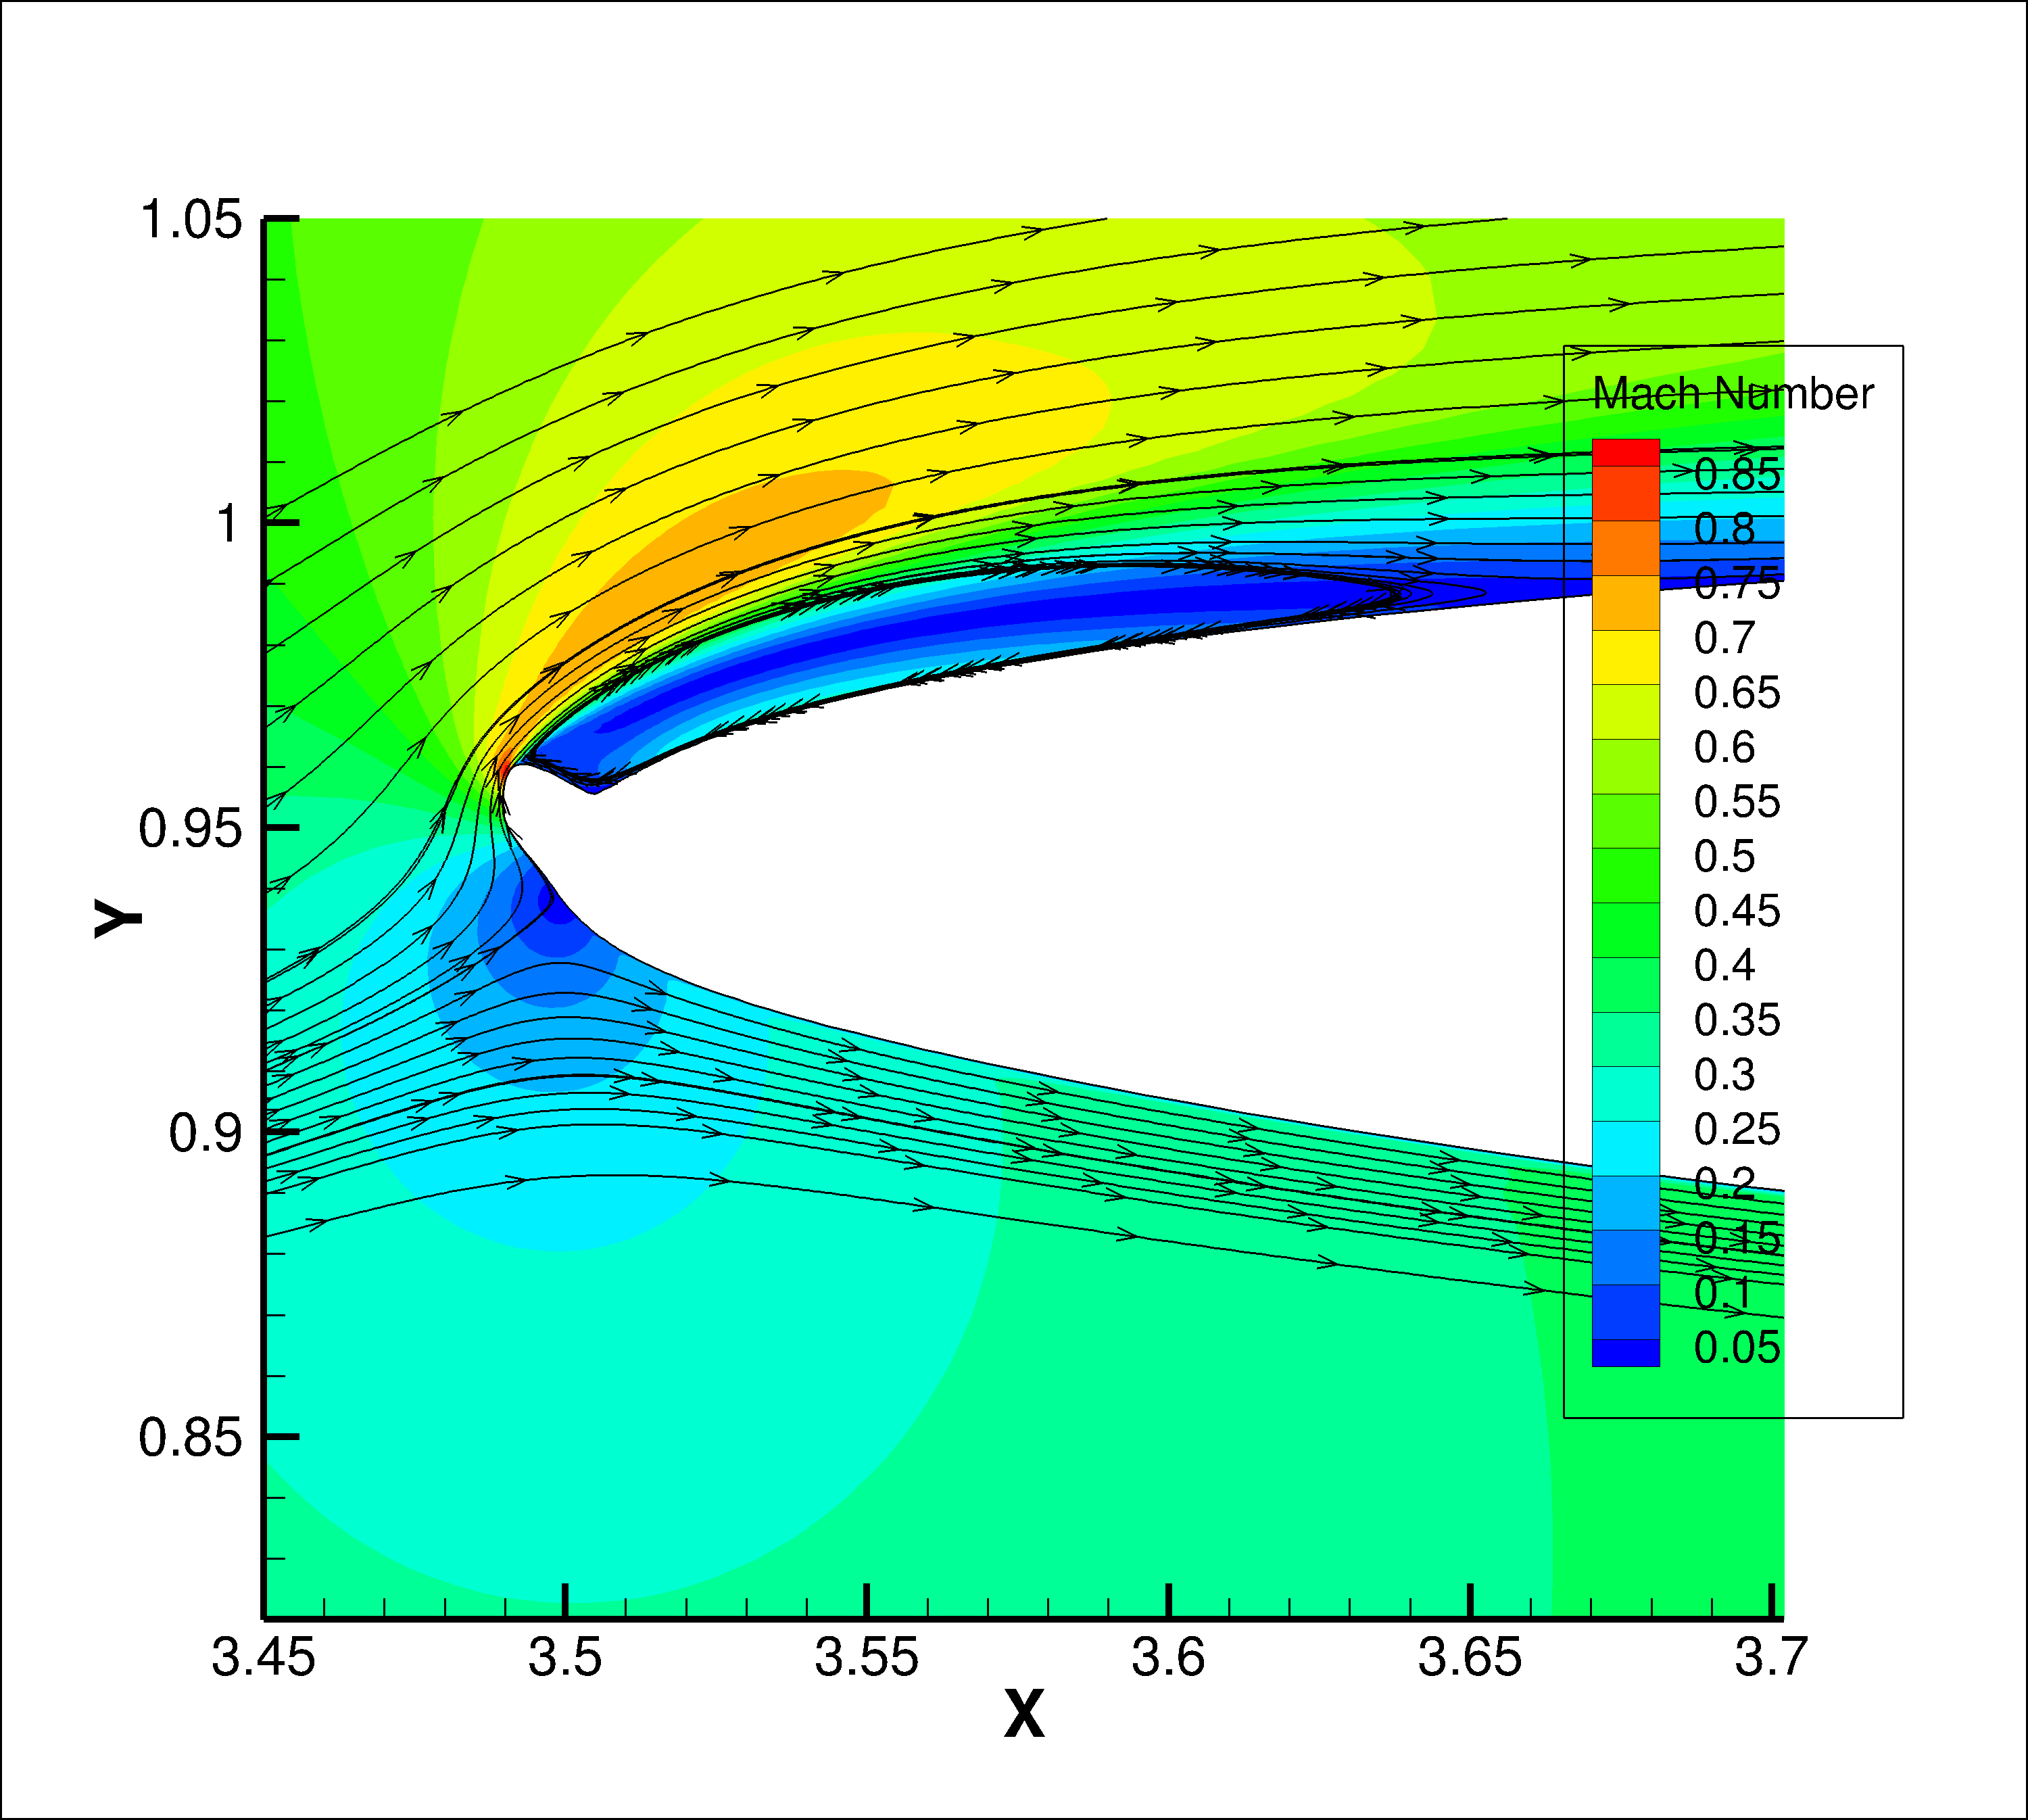
\includegraphics[width=0.4\textwidth]{BadHorn.png}
    \caption{Leading edge horn separation}
\end{figure}
\end{frame}
\begin{frame}
\frametitle{Introduction}
\label{sec-1-2}

\textbf{Significant ice shape variation, sensitivity to physical parameters}\footnote{Addy, H.E. \emph{Ice Accretions and Icing Effects for Modern Airfoils}. NASA TR 2000-210031.
 }
\begin{itemize}
\item Complex physics (aero-thermodynamics, macro/micro scale physics)
\item Uncertainty in physical parameters
\end{itemize}

\vspace*{-0.0cm}\begin{figure}
      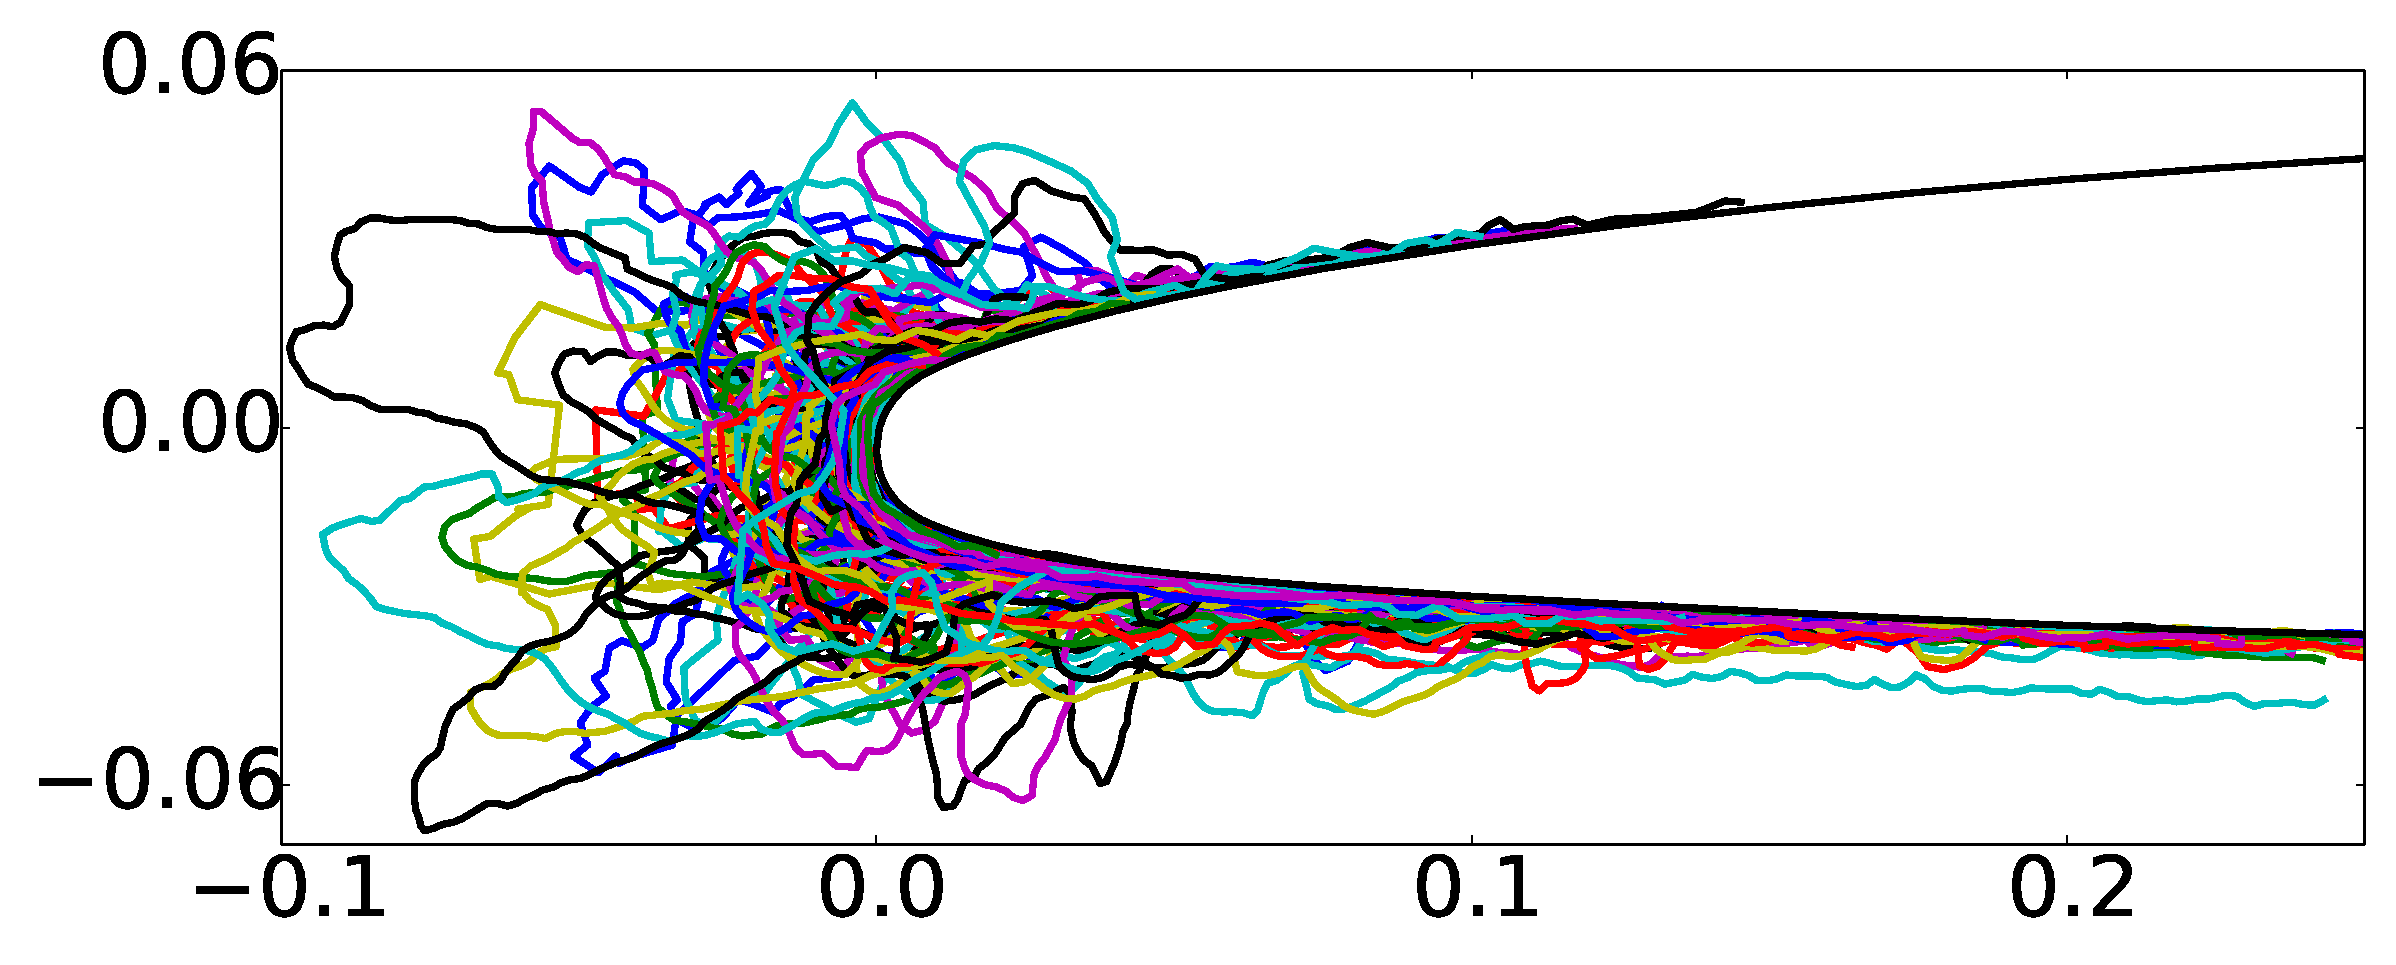
\includegraphics[width=0.75\textwidth]{GlobalDataSet}
      \caption{Wind tunnel experimental ice shapes}
\end{figure}
\end{frame}
\begin{frame}
\frametitle{Introduction}
\label{sec-1-3}

\textbf{Different types of ice accretion}\footnote{Beaugendre et. al. \emph{Development of a Second Generation In-Flight Simulation Code}. J. Fluids Engineering, 2006.
 }
\begin{itemize}
\item ``Horns'', ``ridges'', ``lobster tails'' refer to shape
\item ``Glaze'', ``rime'' refer to icing thermodynamics
\end{itemize}

\vspace*{-0.0cm}\begin{figure}
      \subfigure[Rime Ice]{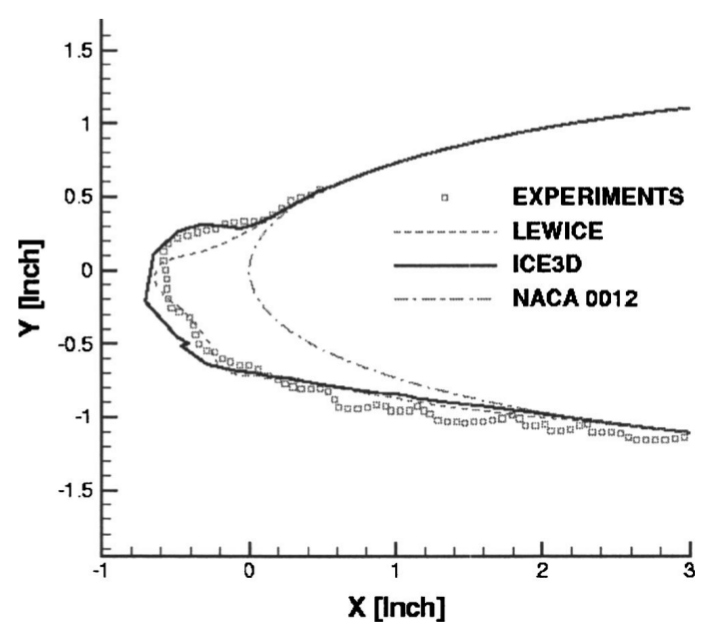
\includegraphics[width=0.4\textwidth]{Habashi2006Rime.png}}
      \subfigure[Horn Ice]{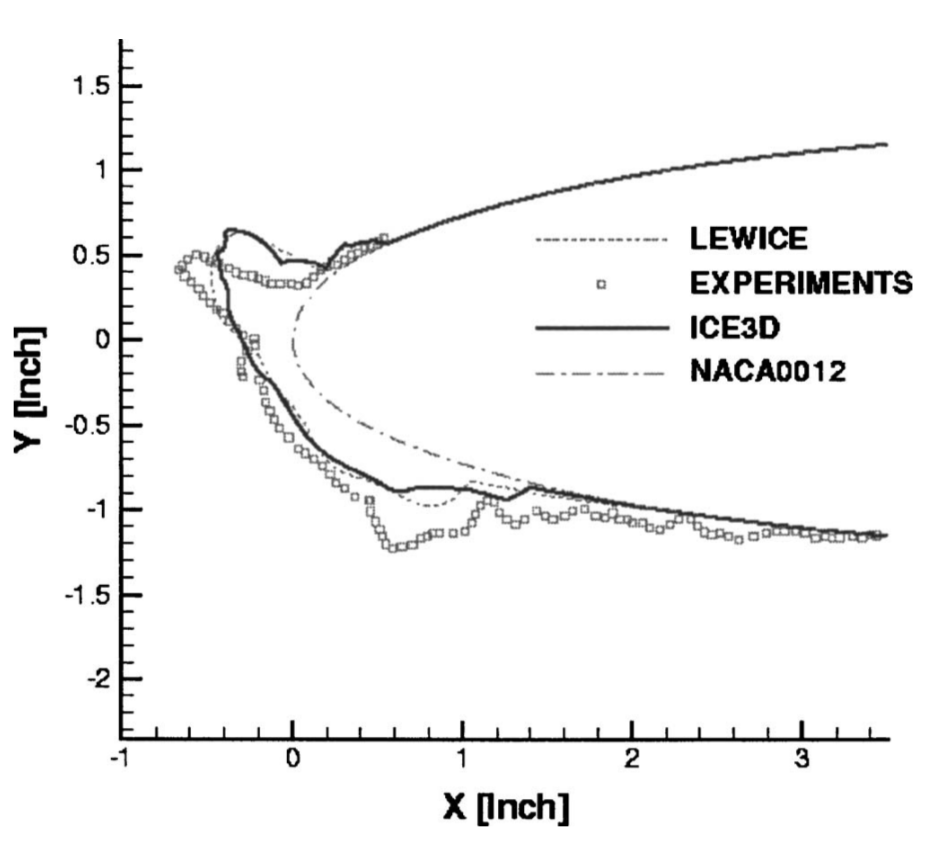
\includegraphics[width=0.4\textwidth]{Habashi2006Horn.png}}
 
\end{figure}
\end{frame}
\begin{frame}
\frametitle{Introduction}
\label{sec-1-4}

\textbf{Research Goals}

\begin{itemize}
\item Data-driven, equation-free model of ice accretion
\begin{itemize}
\item Model ice accretion using \emph{only} data, no physics
\item Study random ice shapes corresponding to a range of icing conditions
\item Could be used to benchmark/correct numerical calculations
\item Could be used to explore \emph{non-deterministic} ice shape variations
\end{itemize}
\item Computational model of ice accretion
\begin{itemize}
\item Build numerical code to calculate ice accretion given physical inputs
\item Compute ice shape for a range of physical conditions
\item Perform parametric UQ and study effects on aerodynamic performance
\end{itemize}
\end{itemize}
\end{frame}
\begin{frame}
\frametitle{Introduction}
\label{sec-1-5}

\textbf{Research Objectives}

\begin{itemize}
\item Data-driven, equation-free modeling of ice accretion
\begin{itemize}
\item Collect large number of ice shapes into a database
\item Model database shape features using Proper Orthogonal Decomposition (POD)
\item Link physical information to shape features
\item Build a purely data-driven, statistical ice accretion model (\emph{no equations})
\item Perform parametric UQ, study performance variations, etc.
\end{itemize}
\item Computational model of ice accretion
\begin{itemize}
\item Build droplet advection/impact simulator (C++)
\item Build icing thermodynamics simulator (C++)
\item Interface code with aerodynamic solver (FLO103)
\item Perform parametric UQ, study performance variations, etc.
\end{itemize}
\end{itemize}
\end{frame}
\section{Data-Based UQ}
\label{sec-2}
\begin{frame}
\frametitle{Dataset}
\label{sec-2-1}

\vspace*{-0.0cm}\begin{figure}
      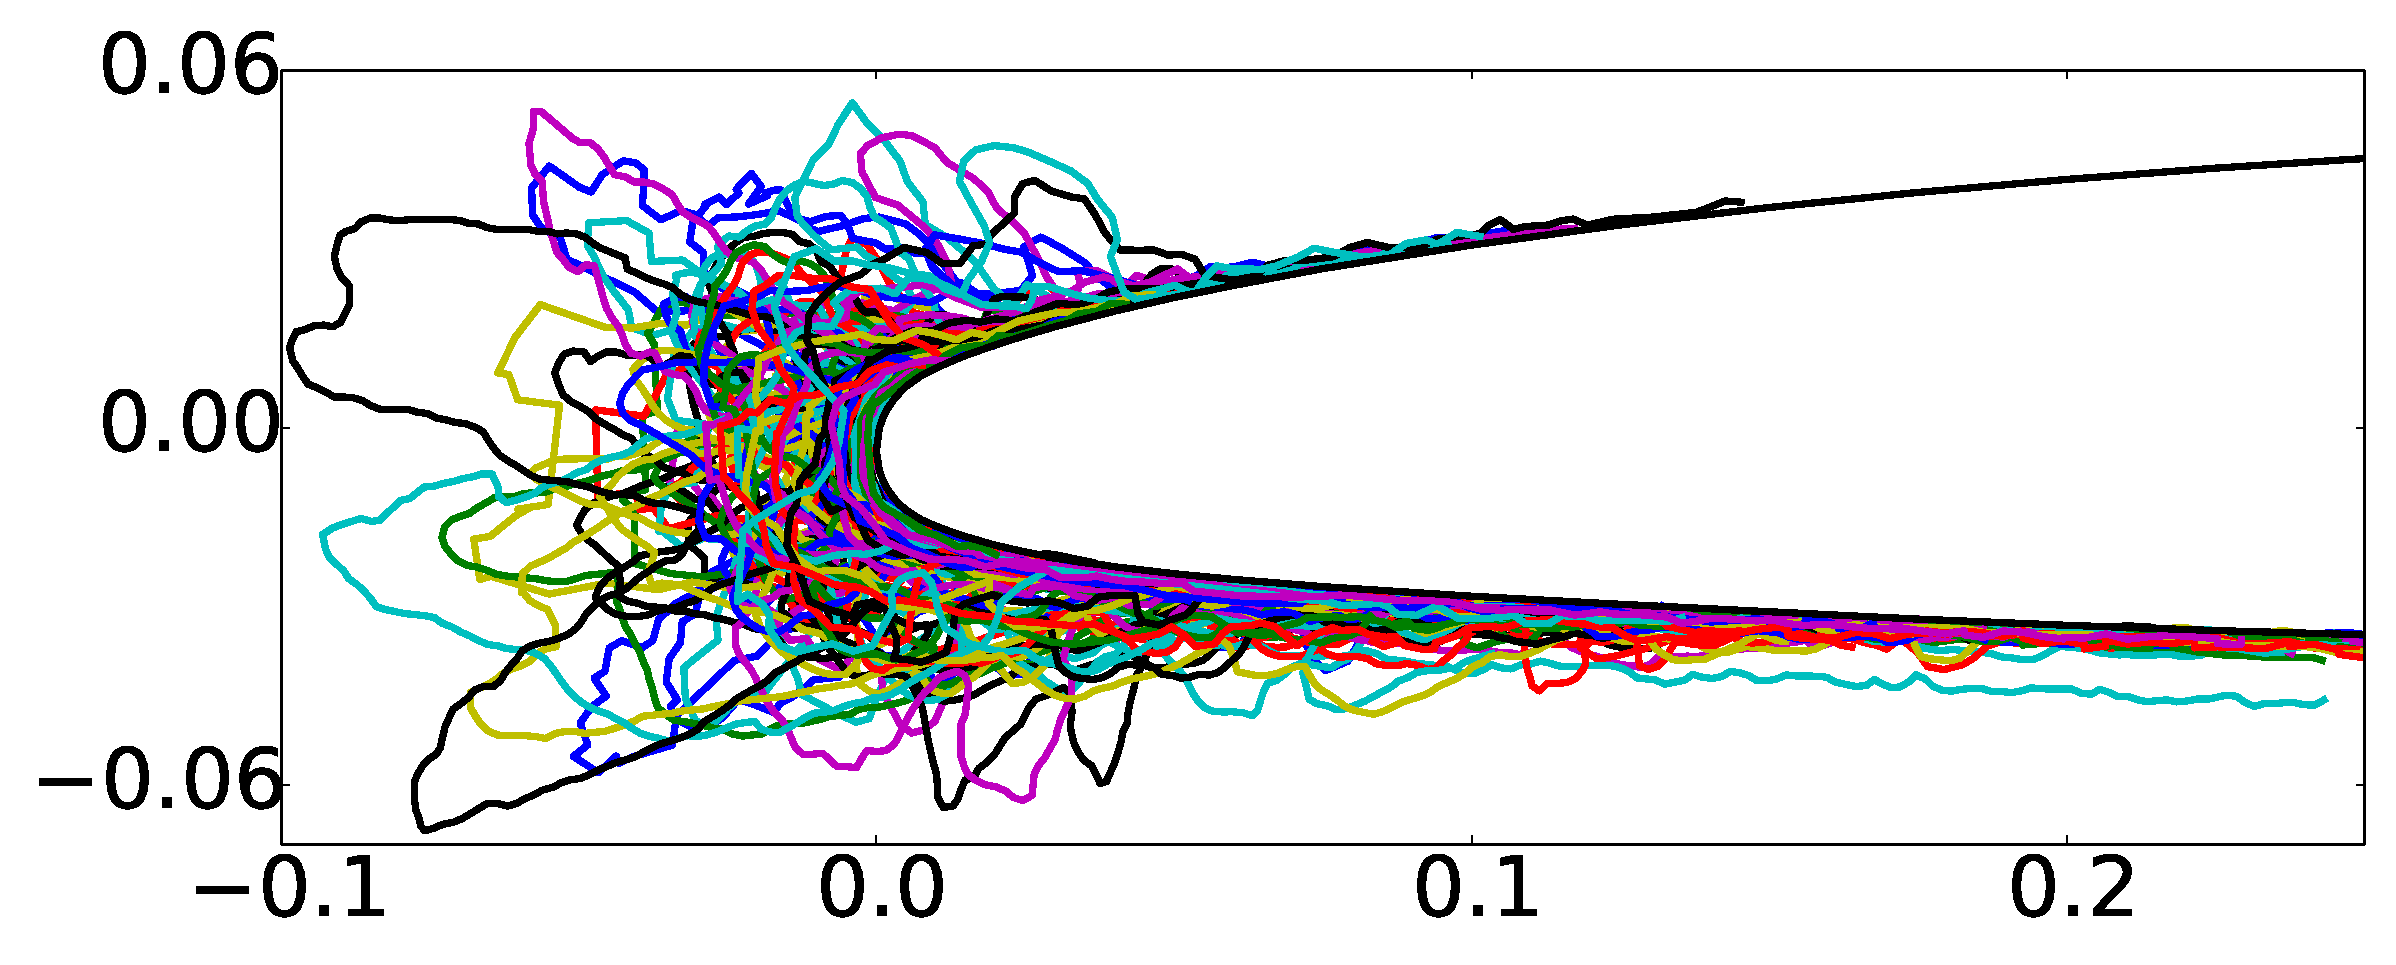
\includegraphics[width=0.5\textwidth]{GlobalDataSet}
      \caption{Wind tunnel experimental ice shapes}
\end{figure}
\begin{itemize}
\item Dataset consists of 145 experimental ice shapes
\item Obtained in icing wind tunnel at NASA Glenn\footnotemark[1]
\item Representative of a wide variety of icing conditions (temperature,
  LWC, accretion time, etc.)
\end{itemize}
\end{frame}
\begin{frame}
\frametitle{Data-Driven Model}
\label{sec-2-2}

\vspace*{-0.0cm}\begin{figure}
      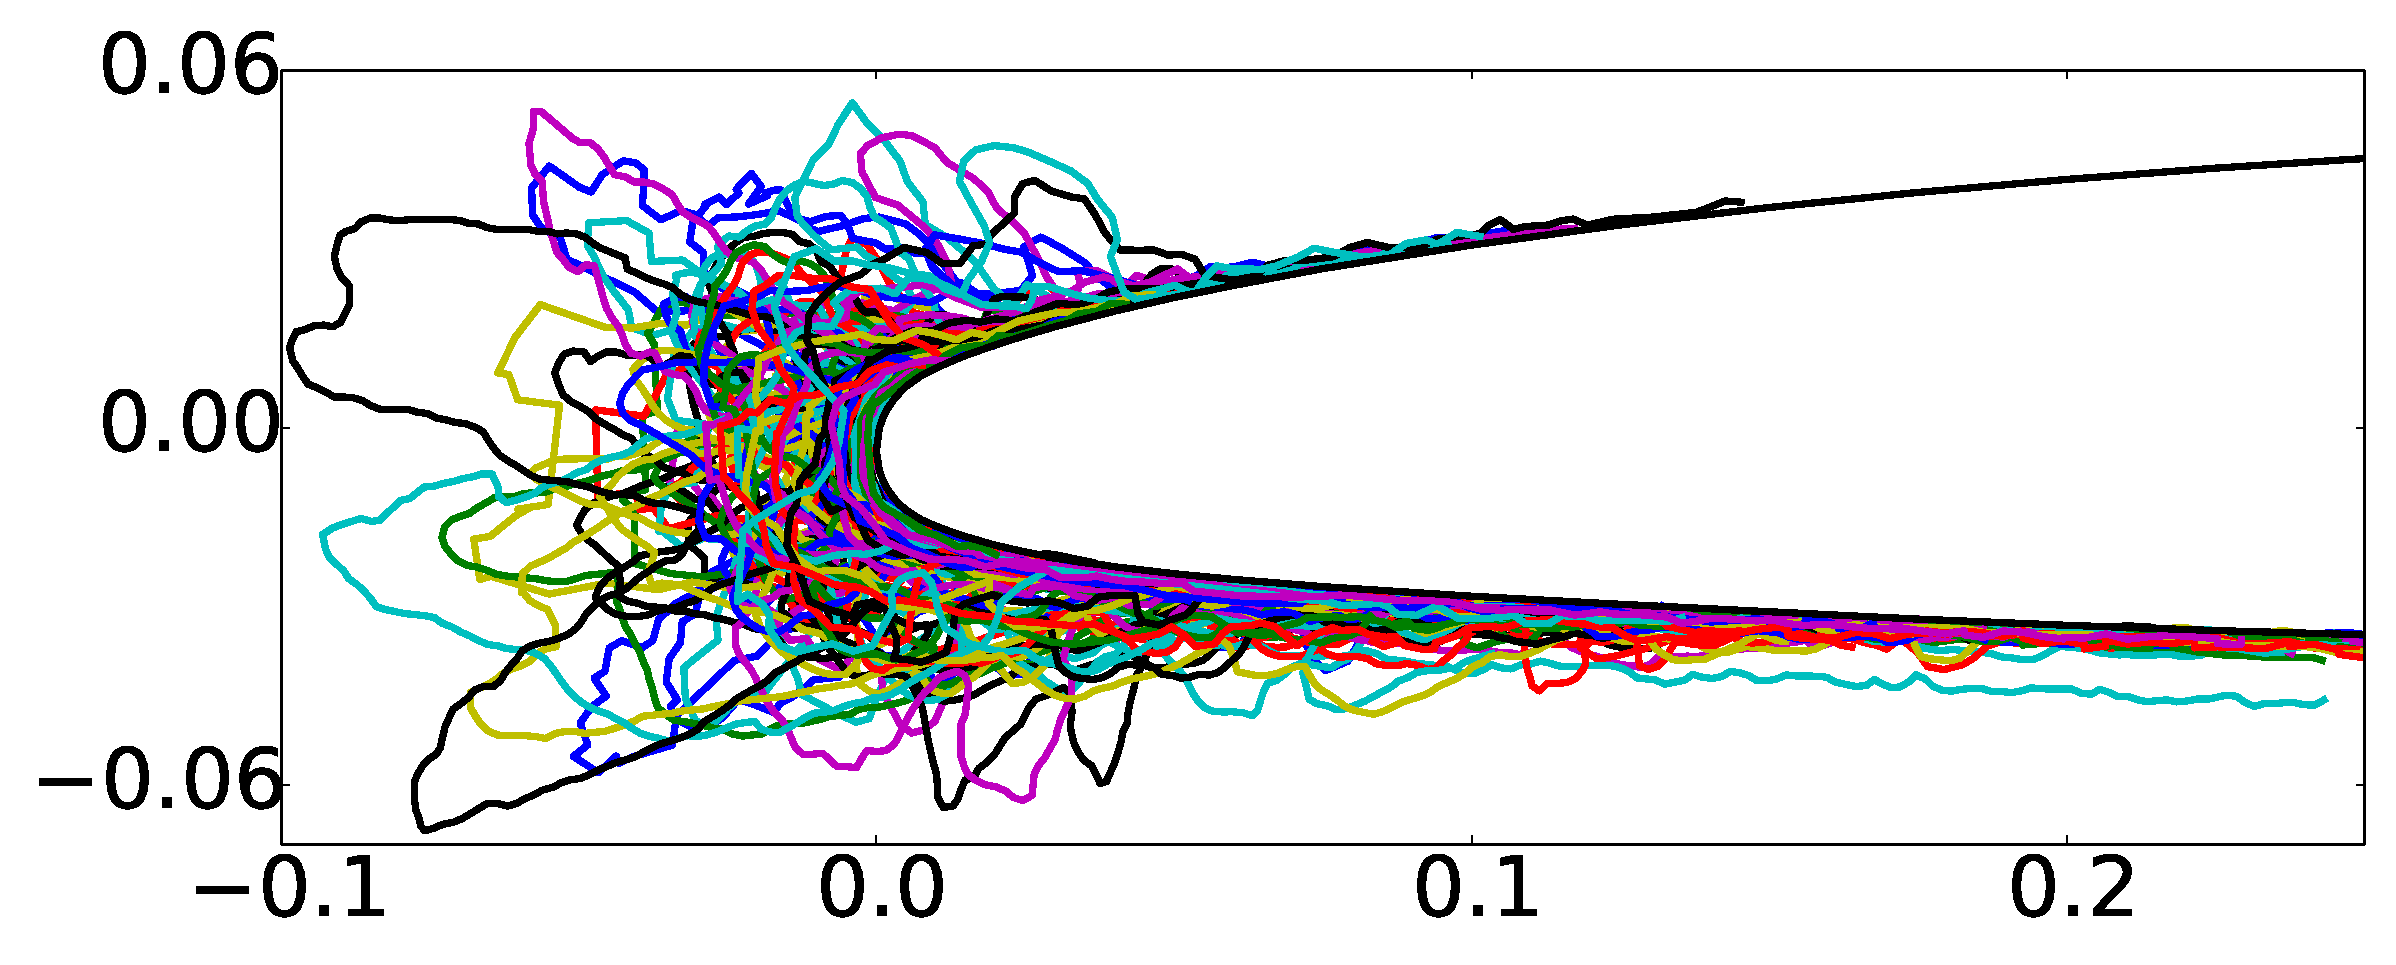
\includegraphics[width=0.5\textwidth]{GlobalDataSet}
      \caption{Wind tunnel experimental ice shapes}
\end{figure}
\textbf{Goal:} Make a purely data-driven model of icing (no equations)

\textbf{Approach:}
\begin{itemize}
\item Build low-dimensional model of shape using POD
\item Correlate POD coefficients to temperature, accretion time, LWC
\item Generate random ice shapes corresponding to given conditions
\begin{itemize}
\item Filter database based on temperature, LWC, time
\item Generate random samples that match POD coefficient statistics
\item Construct corresponding ice shapes
\end{itemize}
\end{itemize}
\end{frame}
\begin{frame}
\frametitle{POD Eigenvalues}
\label{sec-2-3}

\vspace*{-0.0cm}\begin{figure}
      \subfigure[Magnitude.]{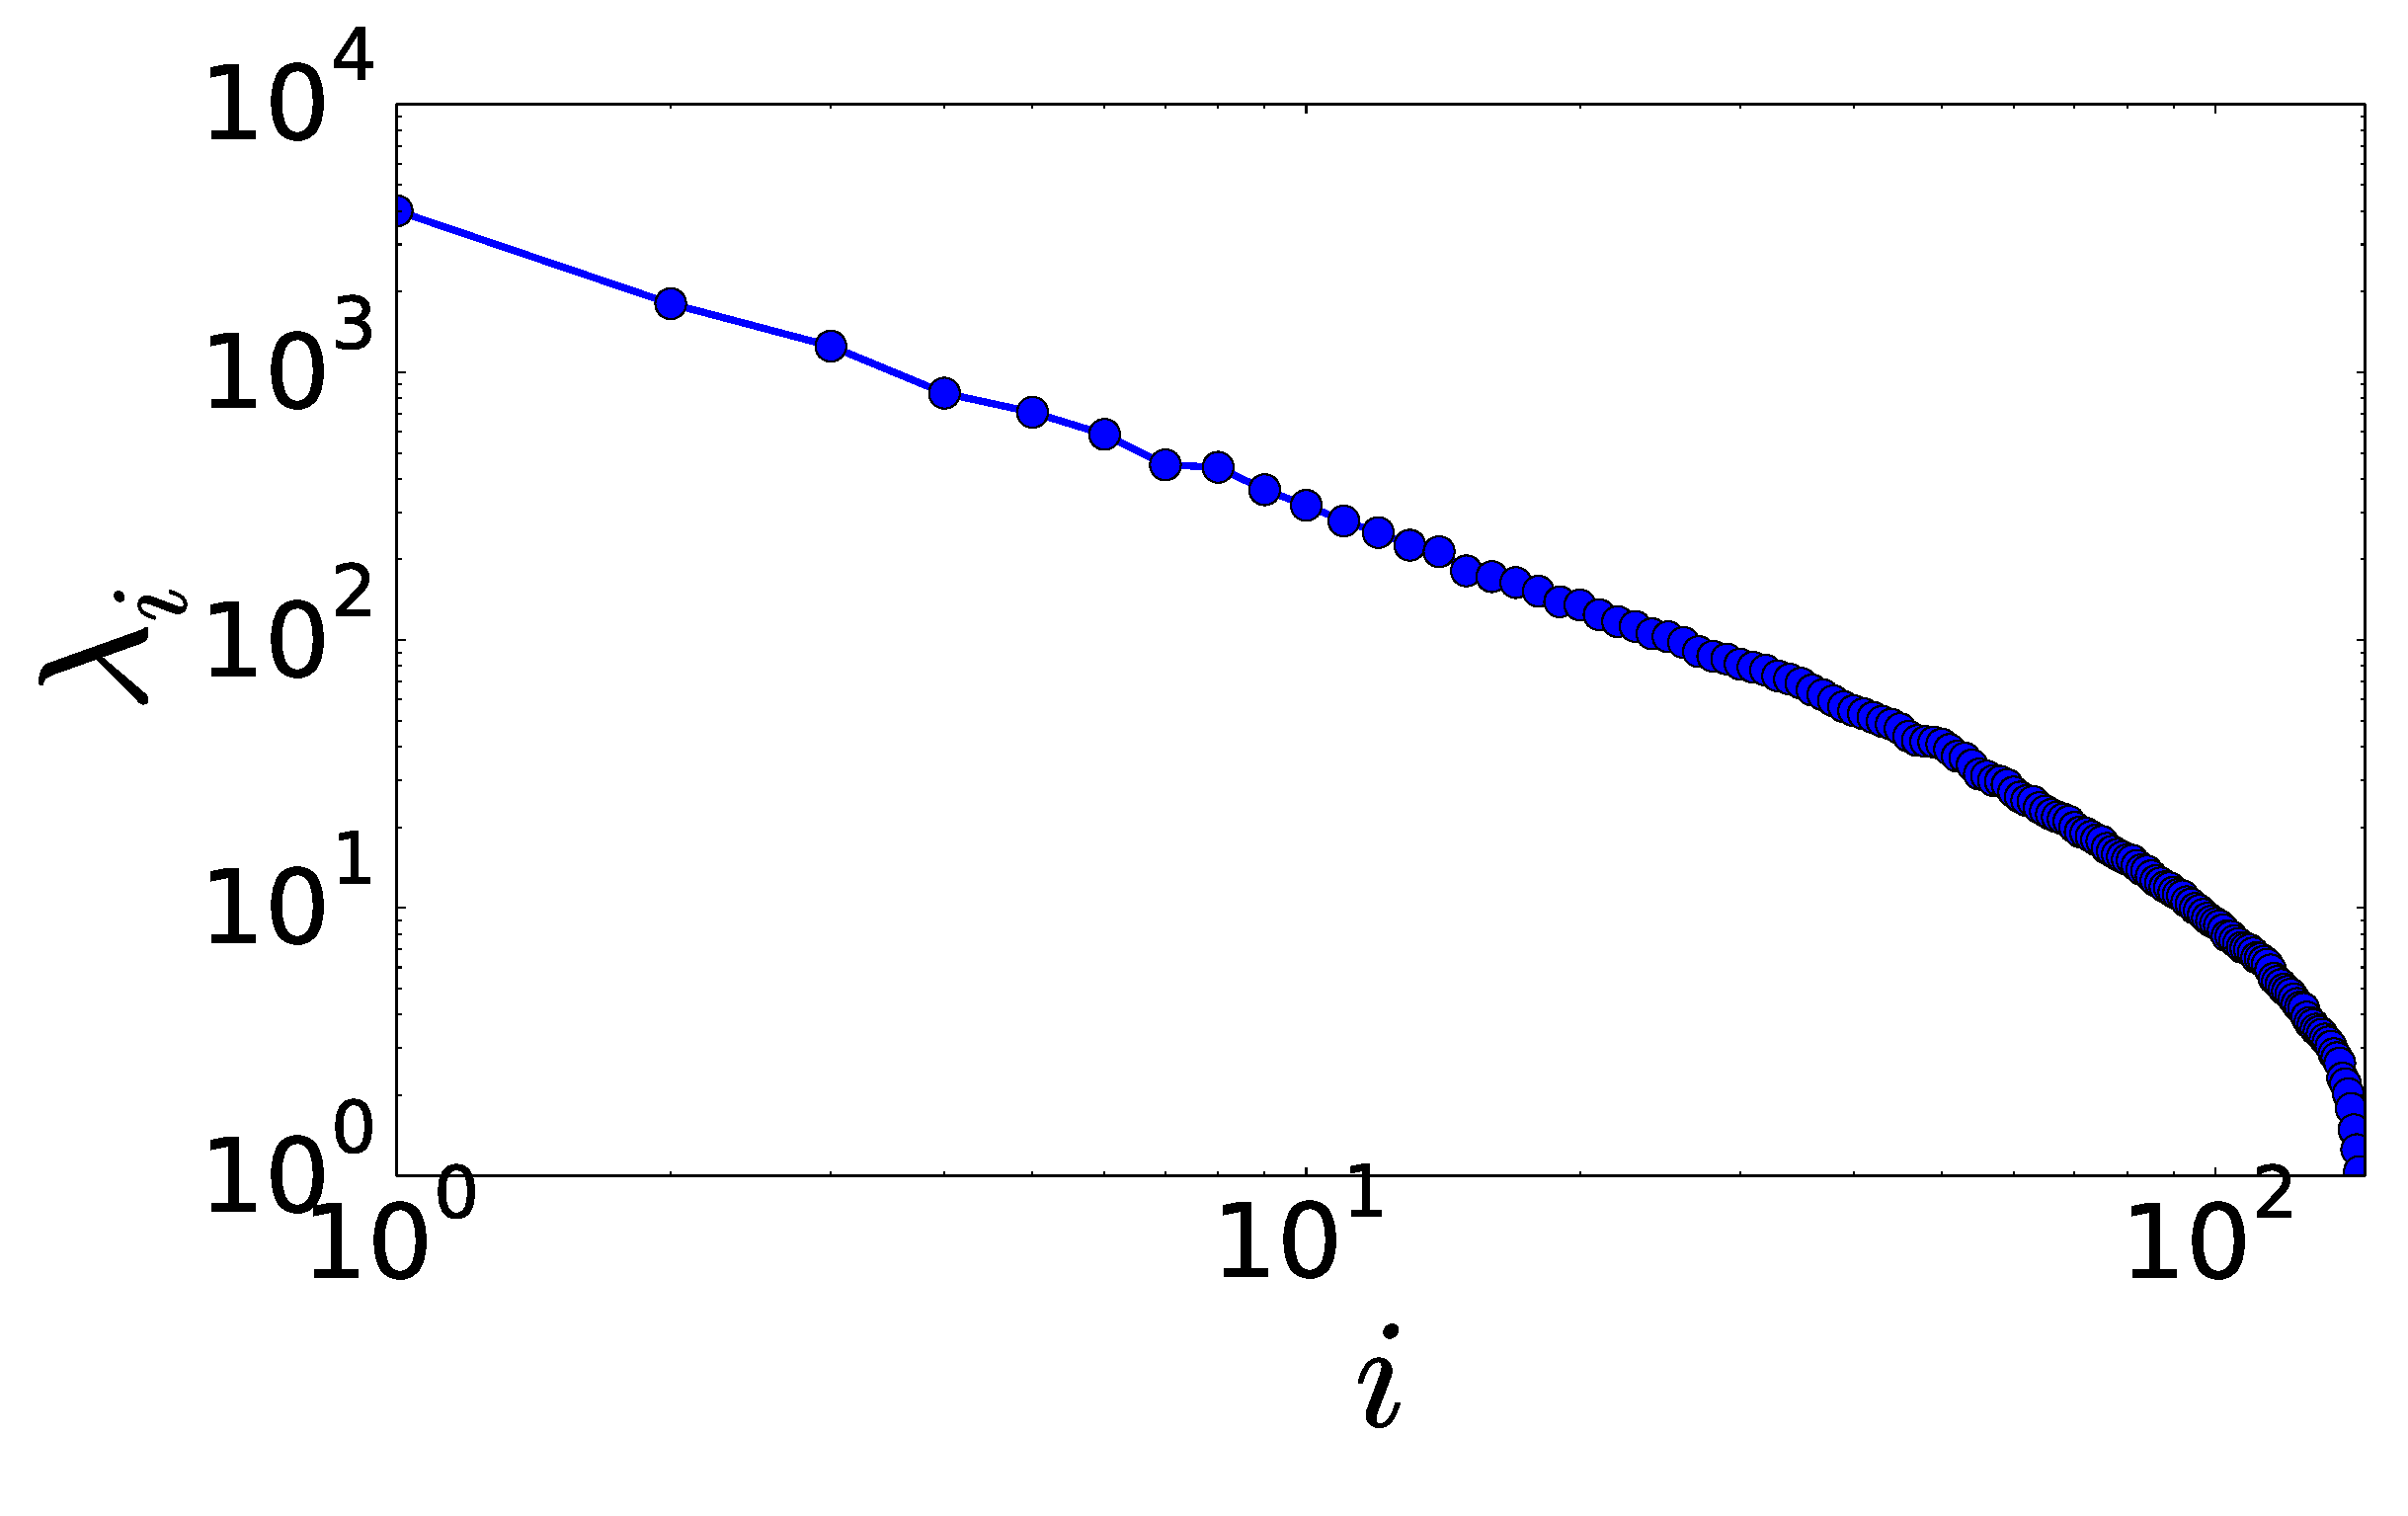
\includegraphics[width=0.4\textwidth]{PODevals.eps}}
      \subfigure[Cumulative sum.]{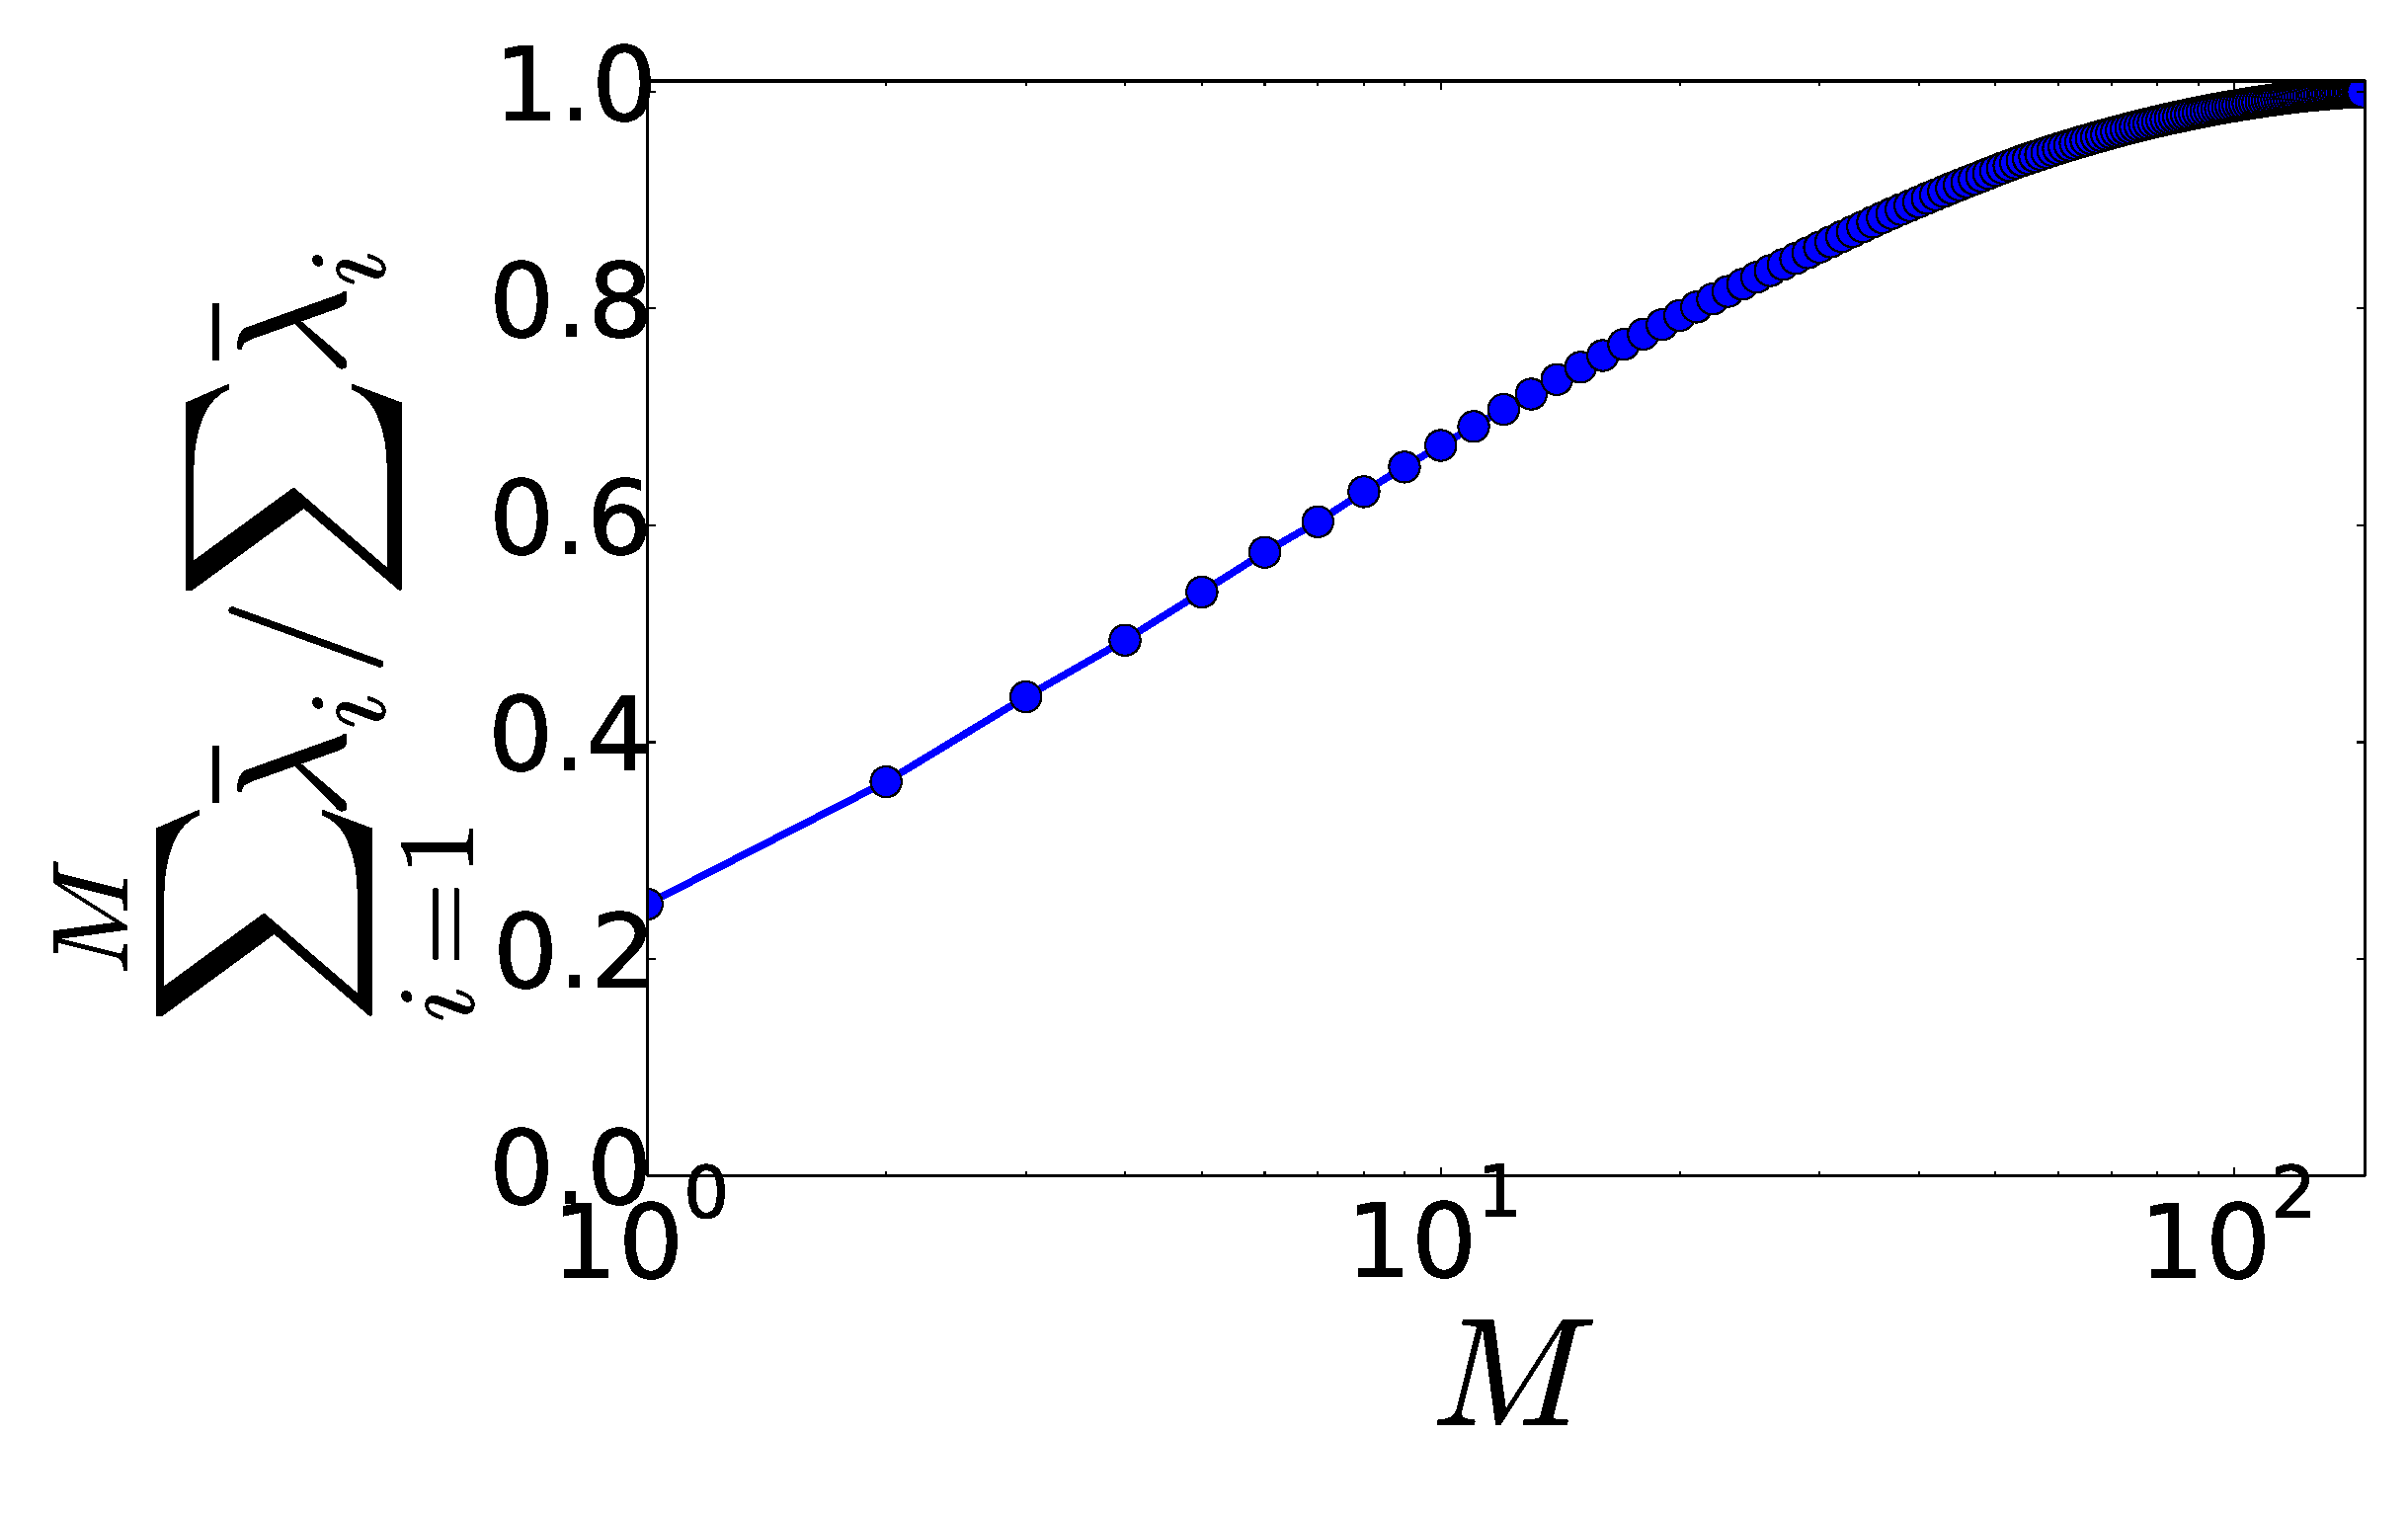
\includegraphics[width=0.4\textwidth]{CumsumPODevals.eps}}
      \caption{POD eigenvalues.}
\end{figure}
\end{frame}
\begin{frame}
\frametitle{POD Modes}
\label{sec-2-4}

\vspace*{-0.0cm}\begin{figure}
      \vspace*{-1.75cm}\subfigure{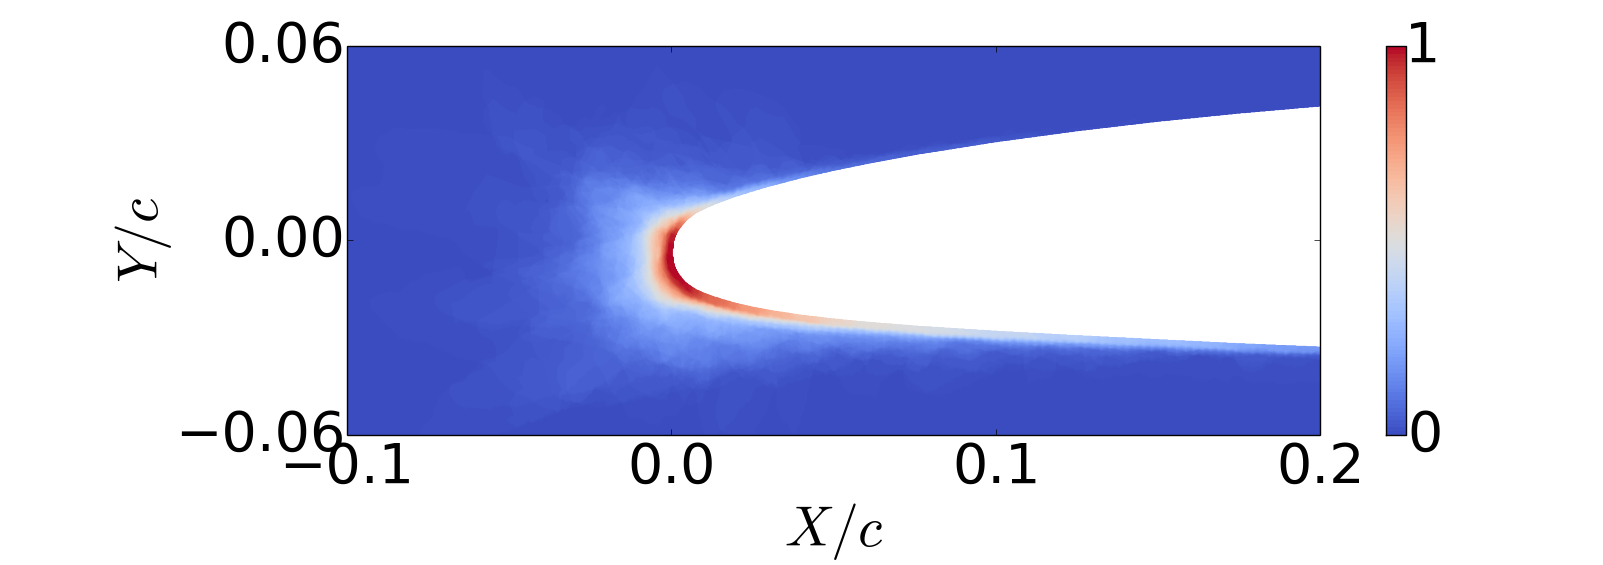
\includegraphics[width=0.4\textwidth]{MEAN}} \\
      \vspace*{-0.75cm}\subfigure{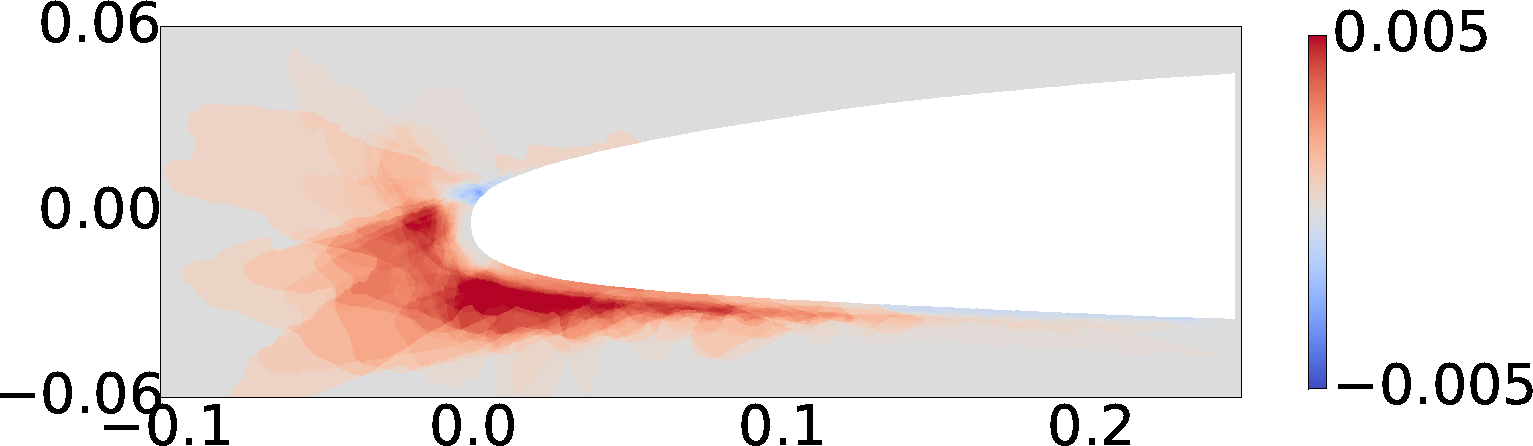
\includegraphics[width=0.4\textwidth]{MODE1}}
      \vspace*{-0.75cm}\subfigure{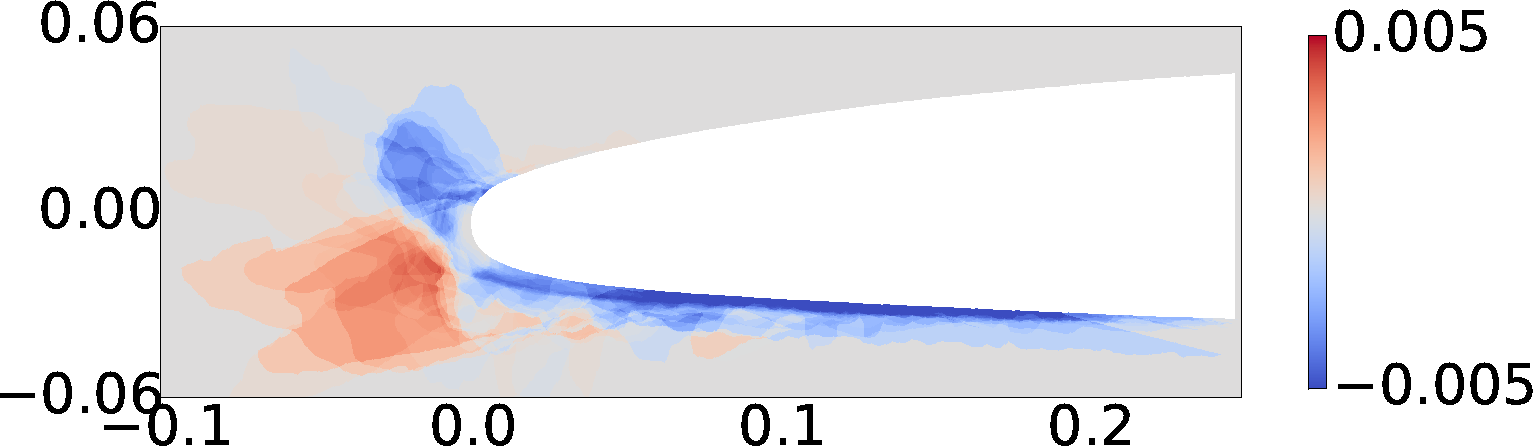
\includegraphics[width=0.4\textwidth]{MODE2}}
      \vspace*{-0.75cm}\subfigure{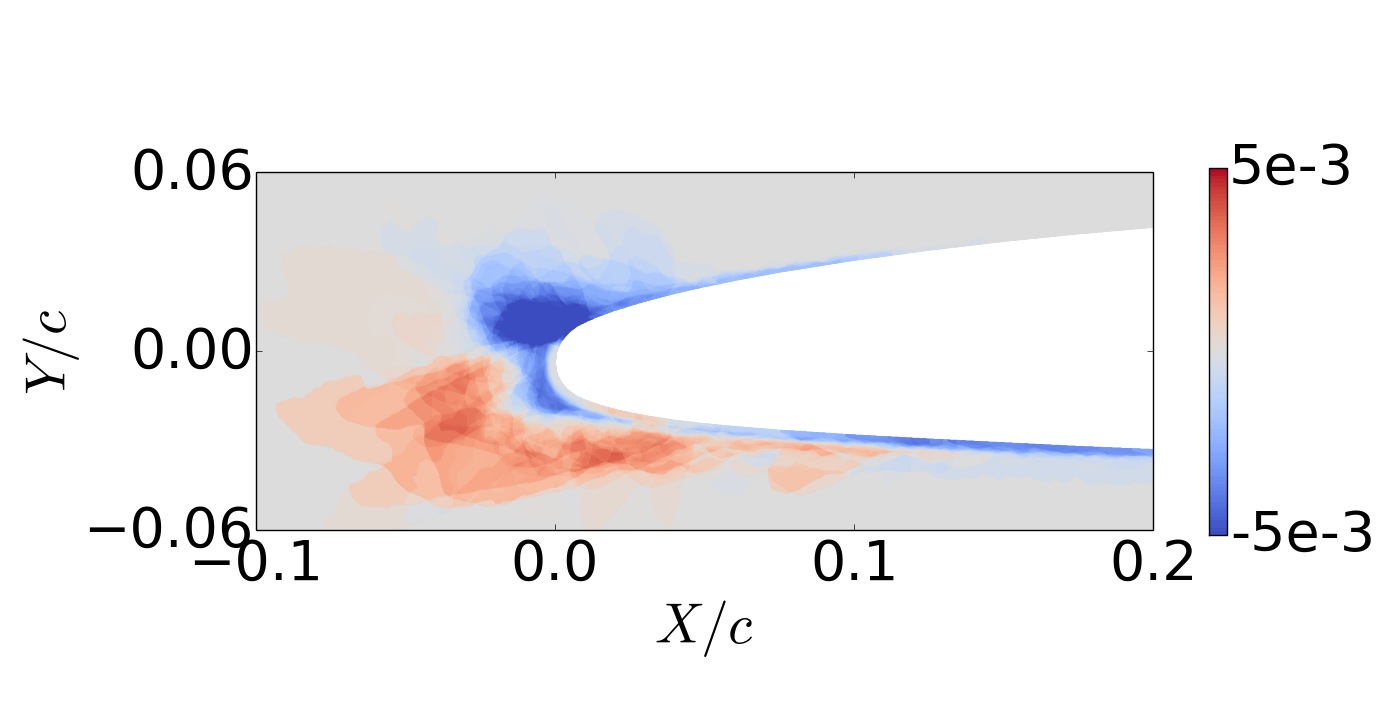
\includegraphics[width=0.4\textwidth]{MODE3}}
      \vspace*{-0.75cm}\subfigure{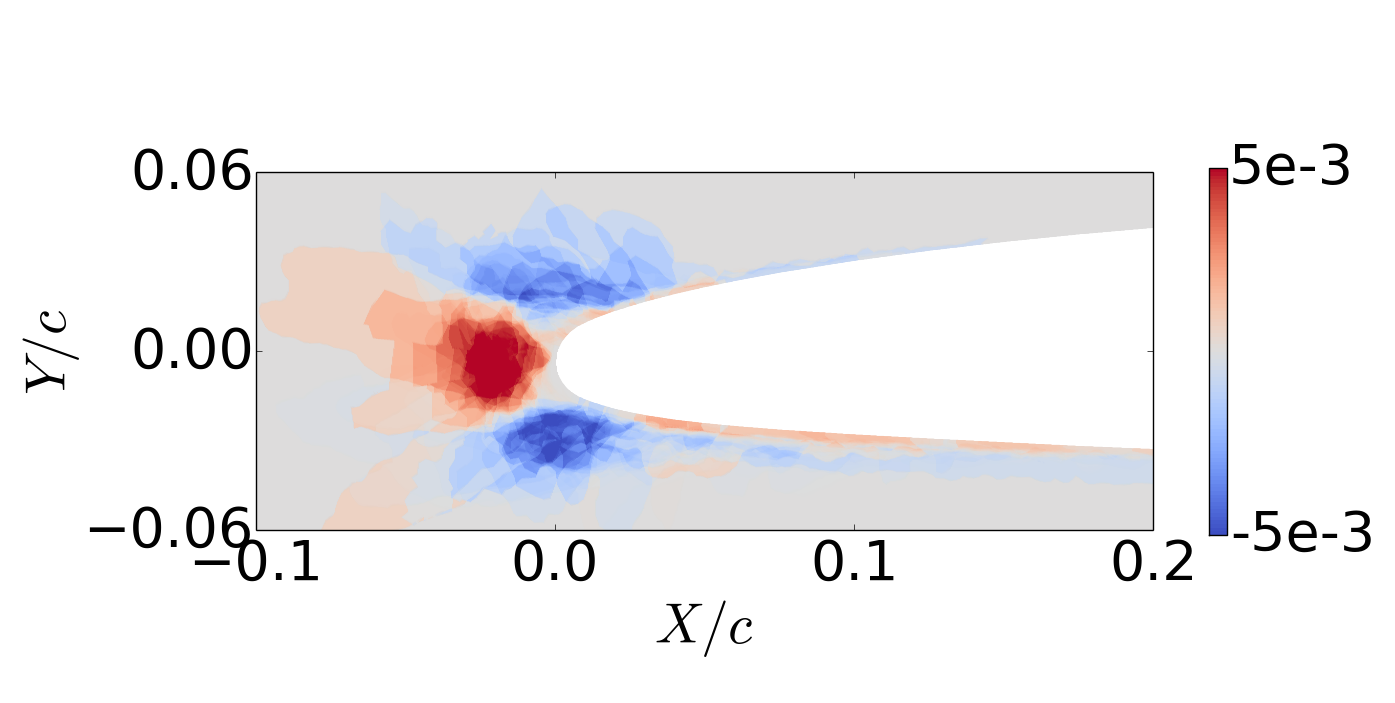
\includegraphics[width=0.4\textwidth]{MODE4}}
      \vspace*{1cm}\caption{Mean and POD modes.}
\end{figure}
\end{frame}
\begin{frame}
\frametitle{POD Reconstructions}
\label{sec-2-5}

\begin{figure}
      \vspace*{-0.9cm}\subfigure{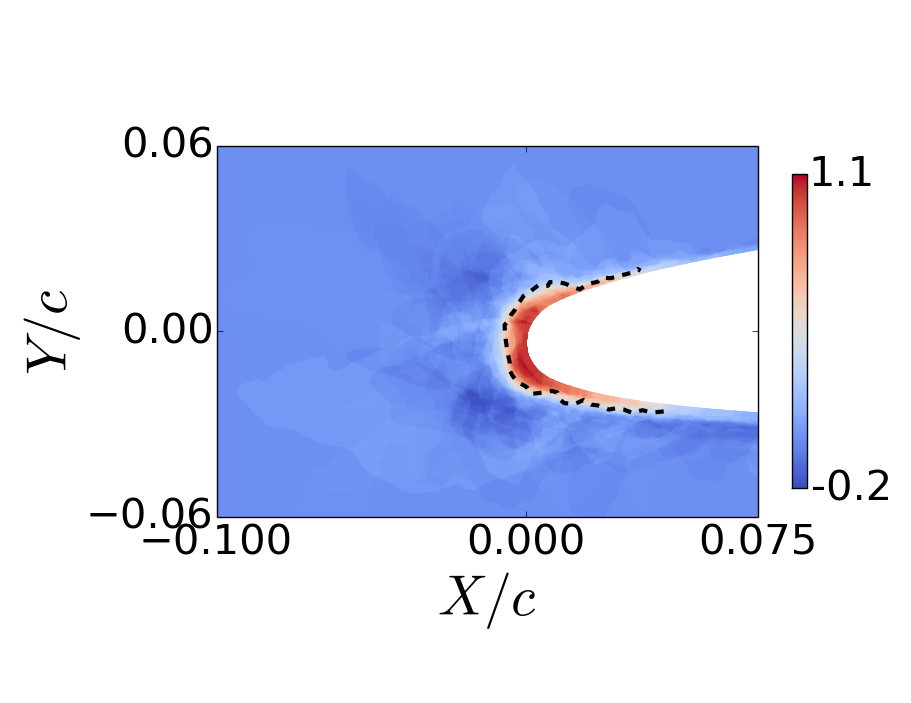
\includegraphics[width=0.35\textwidth]{UnfilteredReconstructionEx2.png}}
      \vspace*{-0.9cm}\subfigure{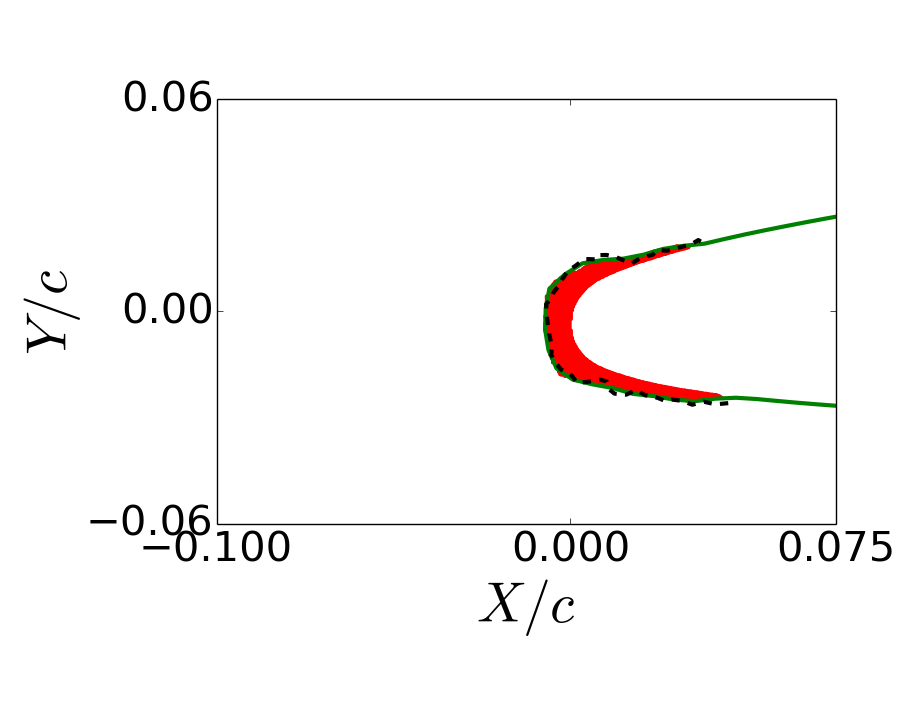
\includegraphics[width=0.35\textwidth]{FilteredReconstructionEx2.png}} \\
      \vspace*{-0.5cm}\subfigure{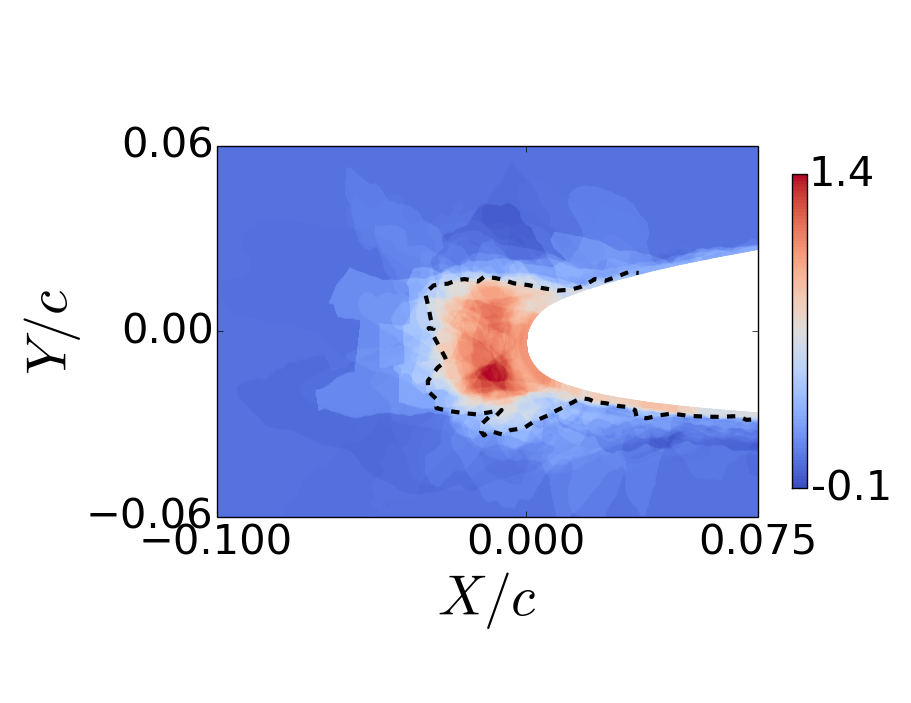
\includegraphics[width=0.35\textwidth]{UnfilteredReconstructionEx3.png}}
      \vspace*{-0.5cm}\subfigure{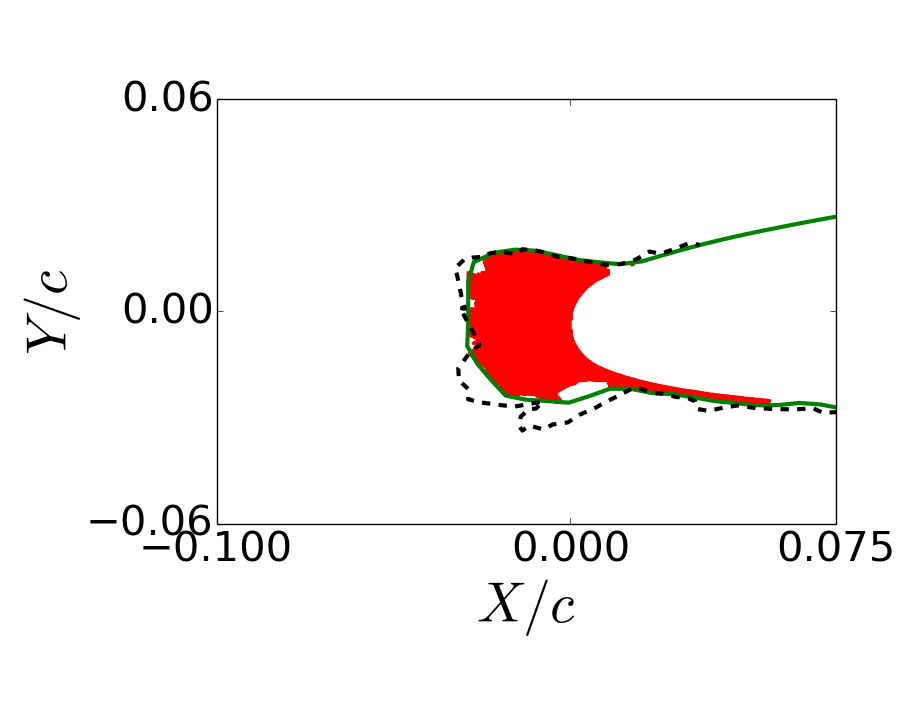
\includegraphics[width=0.35\textwidth]{FilteredReconstructionEx3.png}} \\
      \vspace*{-0.5cm}\subfigure{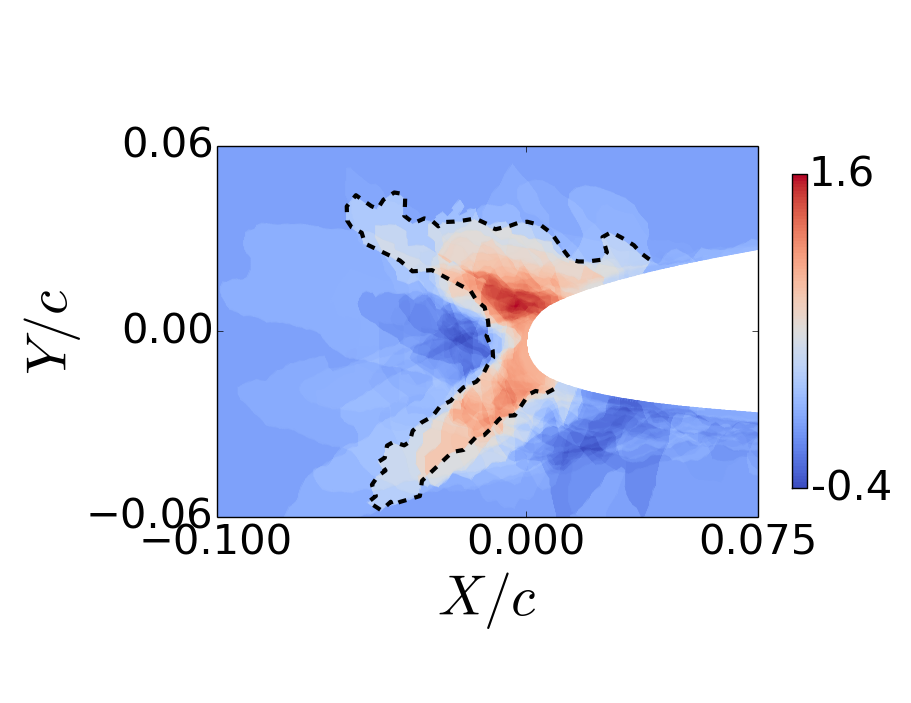
\includegraphics[width=0.35\textwidth]{UnfilteredReconstructionEx1.png}}
      \vspace*{-0.5cm}\subfigure{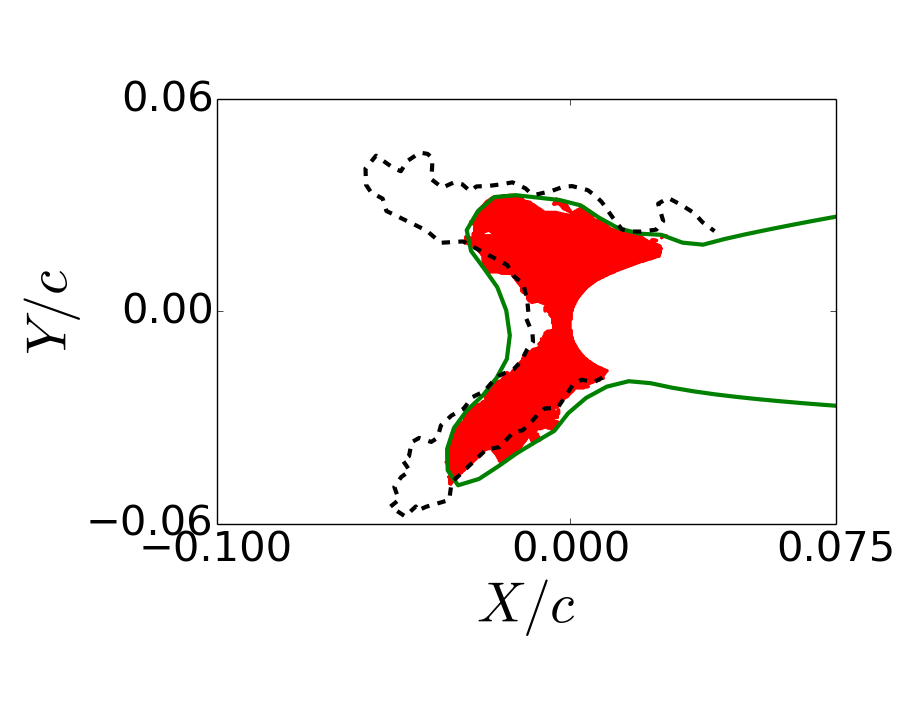
\includegraphics[width=0.35\textwidth]{FilteredReconstructionEx1.png}}
      \vspace*{0cm}\caption{POD reconstructions.}
\end{figure}
\end{frame}
\begin{frame}
\frametitle{Link Physical Conditions to Modes}
\label{sec-2-6}

\begin{figure}
      \vspace*{-0.4cm}\subfigure{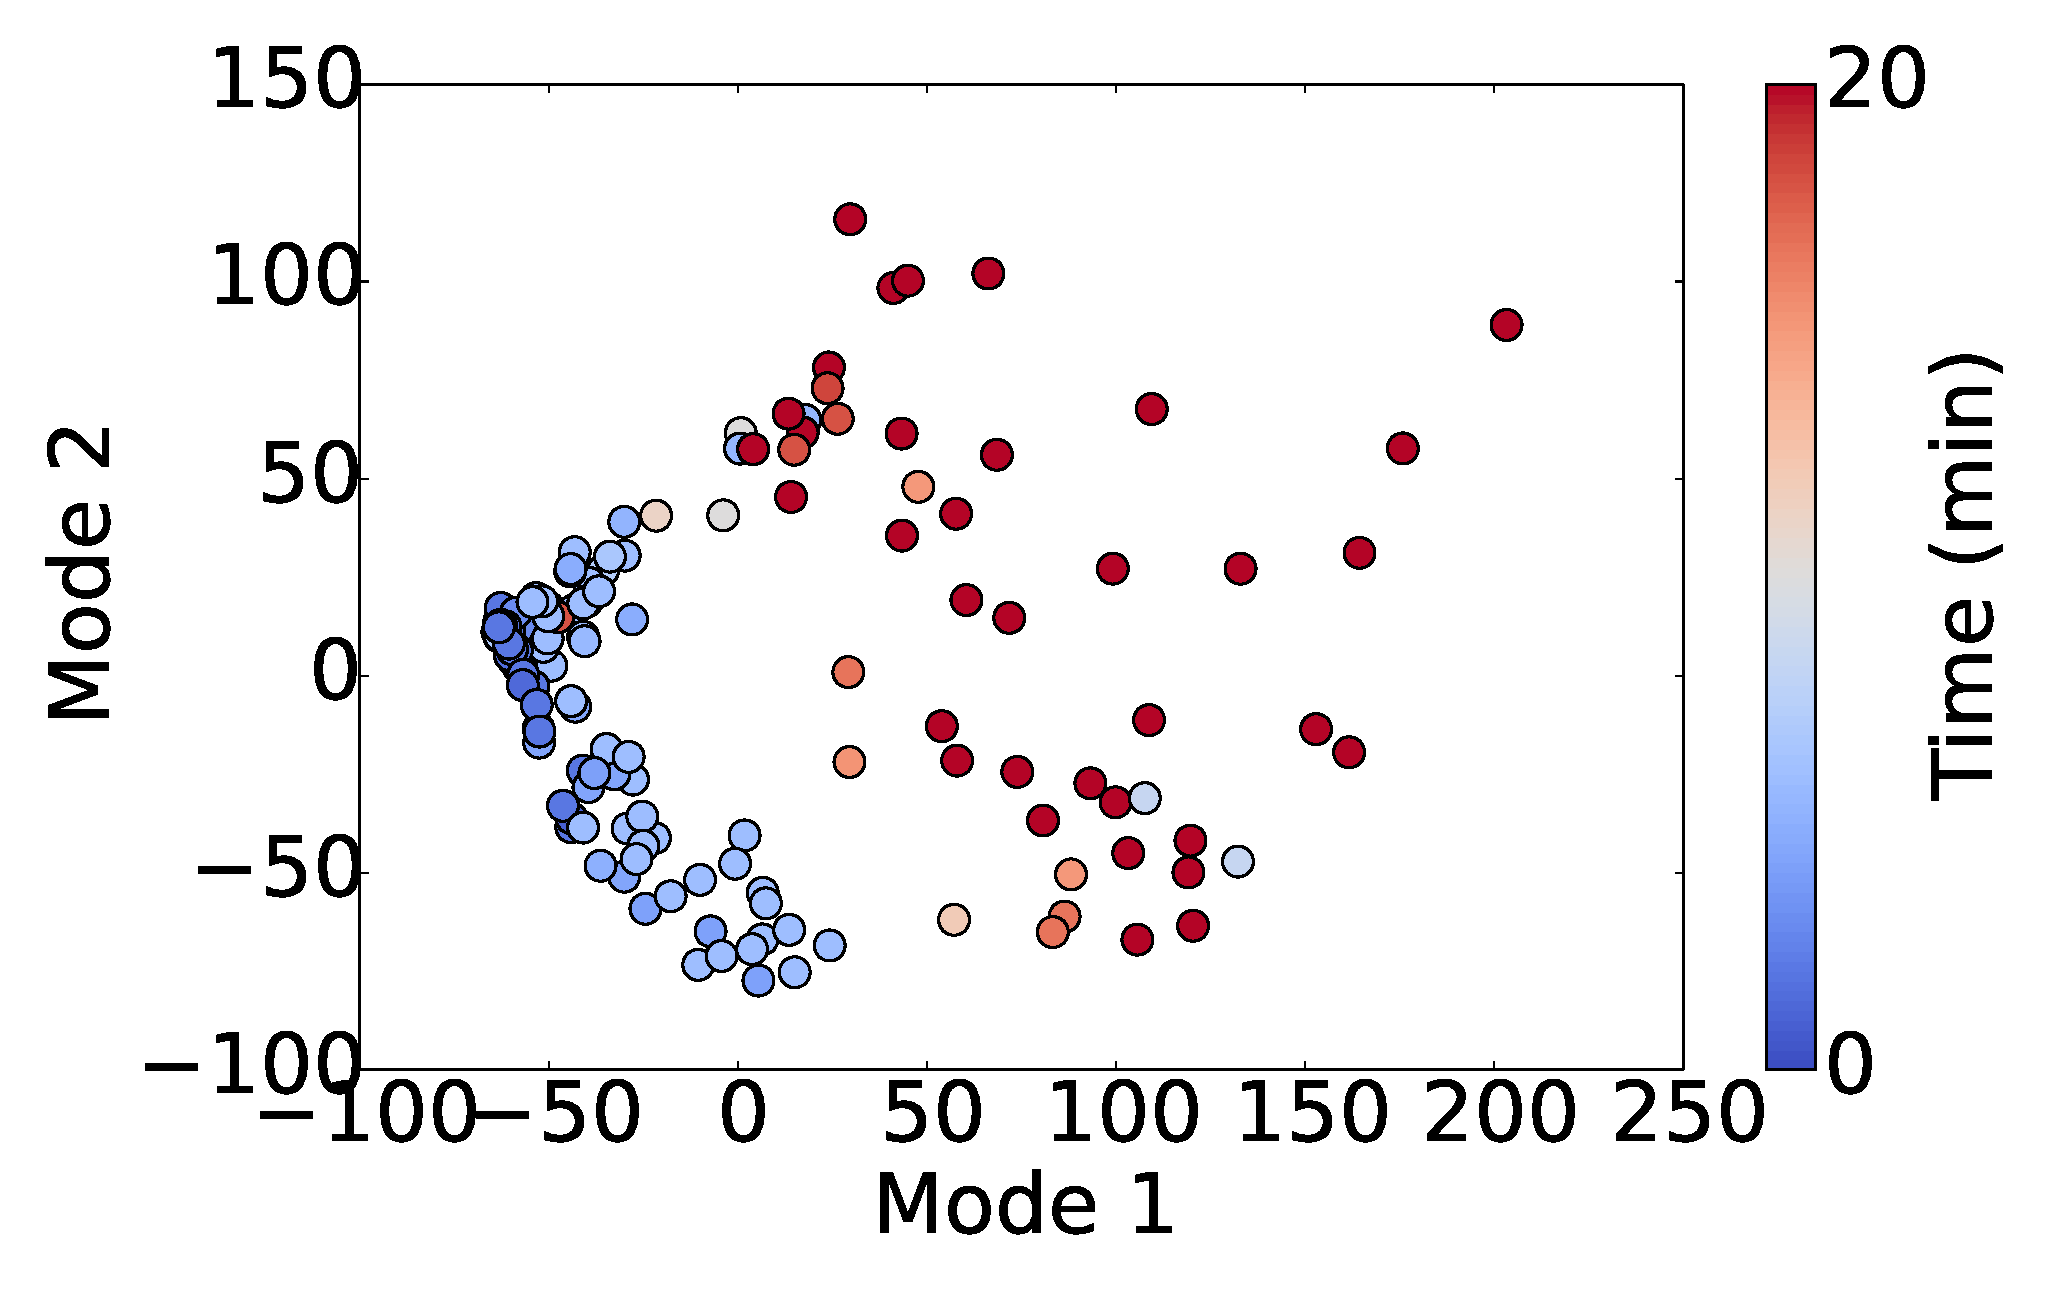
\includegraphics[width=0.4\textwidth]{10ParamMode1Mode2Time}}
      \vspace*{-0.4cm}\subfigure{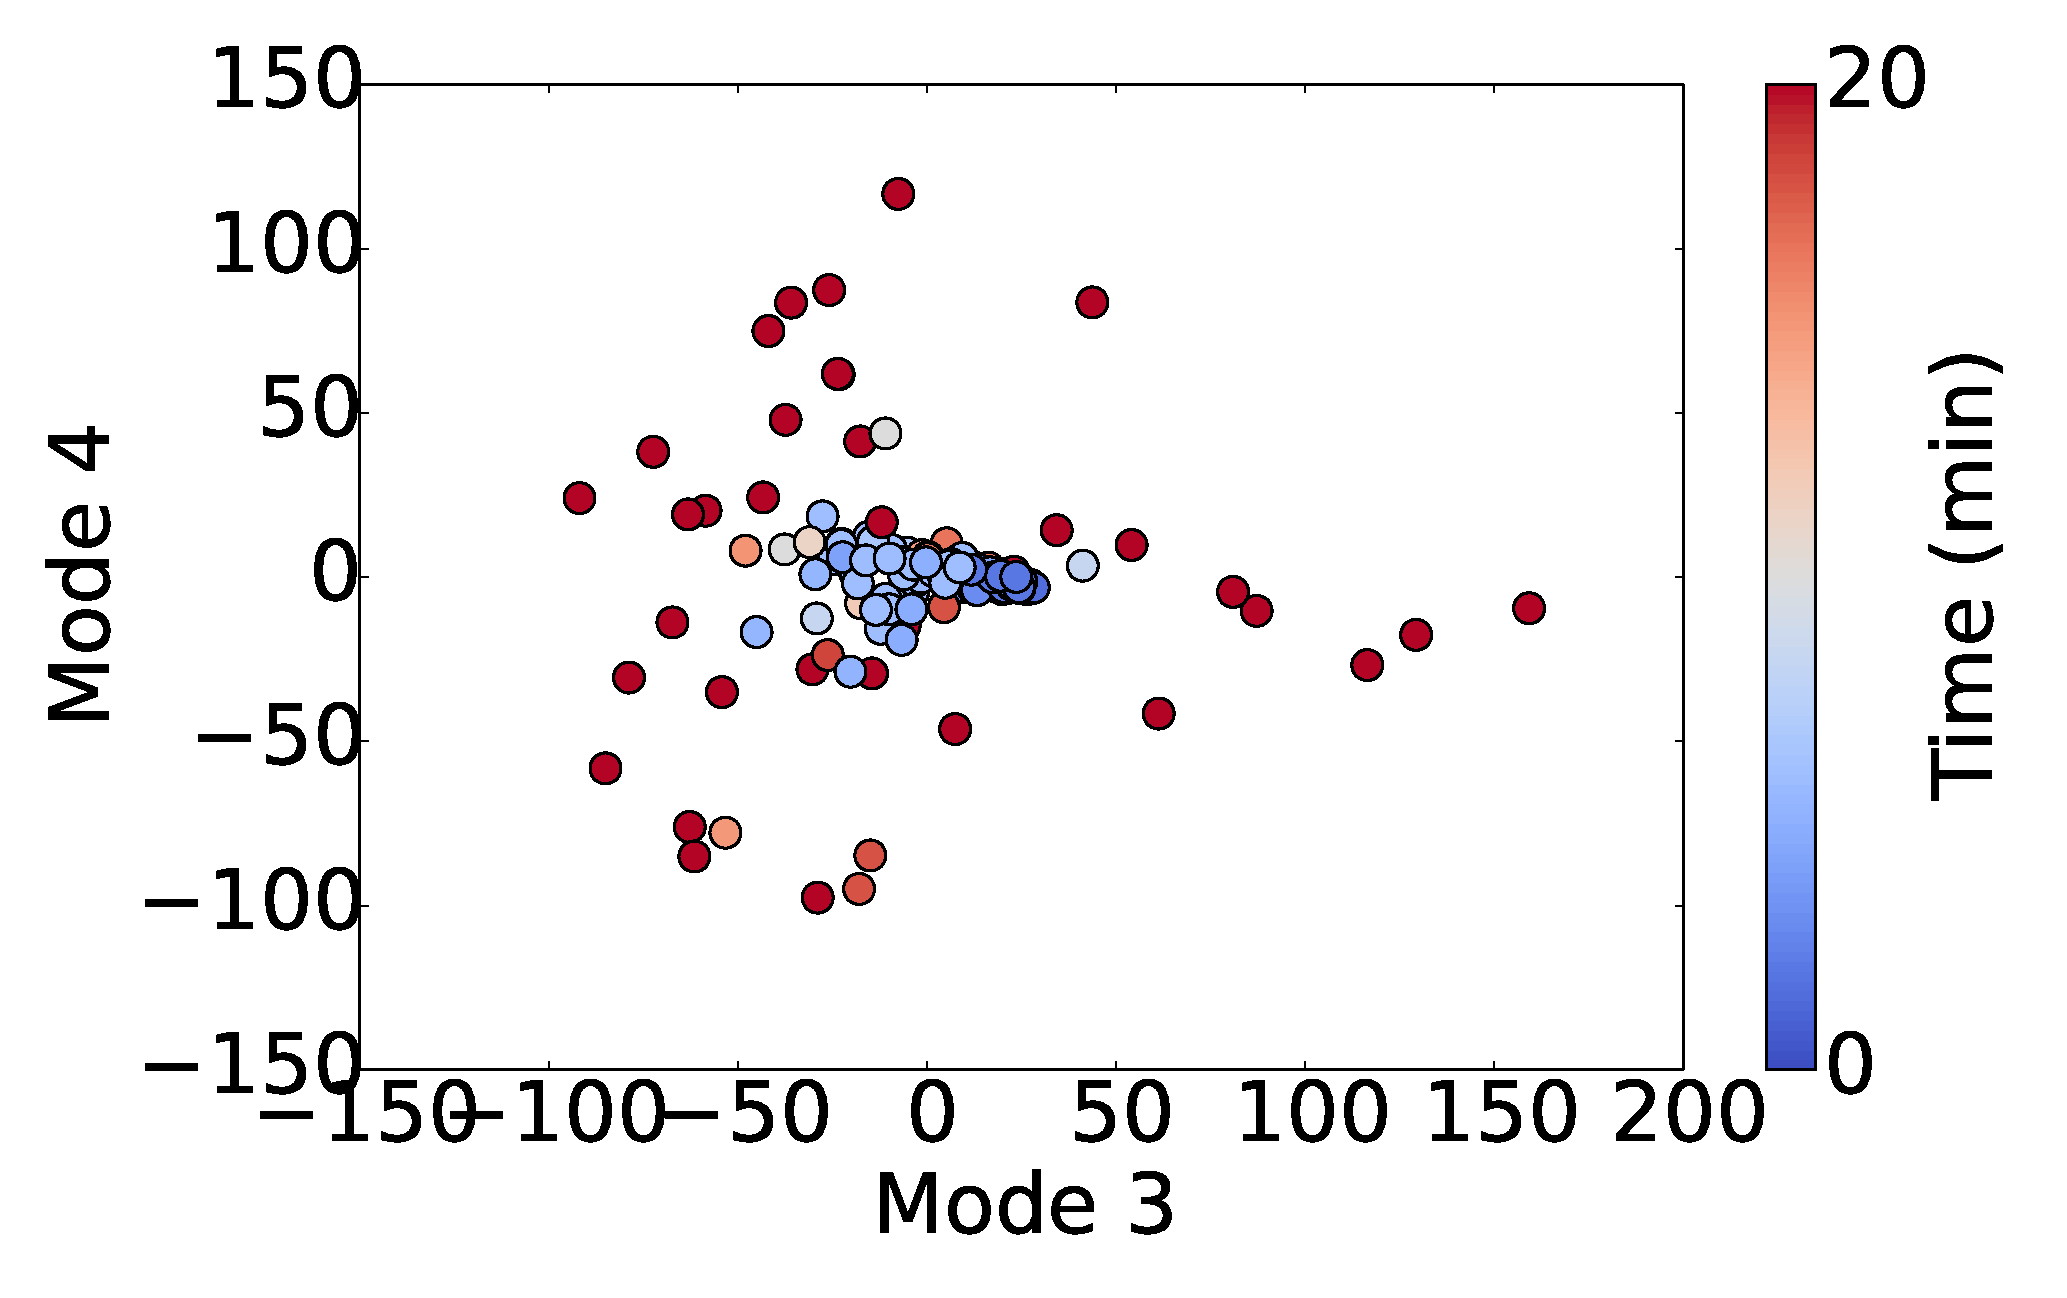
\includegraphics[width=0.4\textwidth]{10ParamMode3Mode4Time}} \\
      \vspace*{-0.4cm}\subfigure{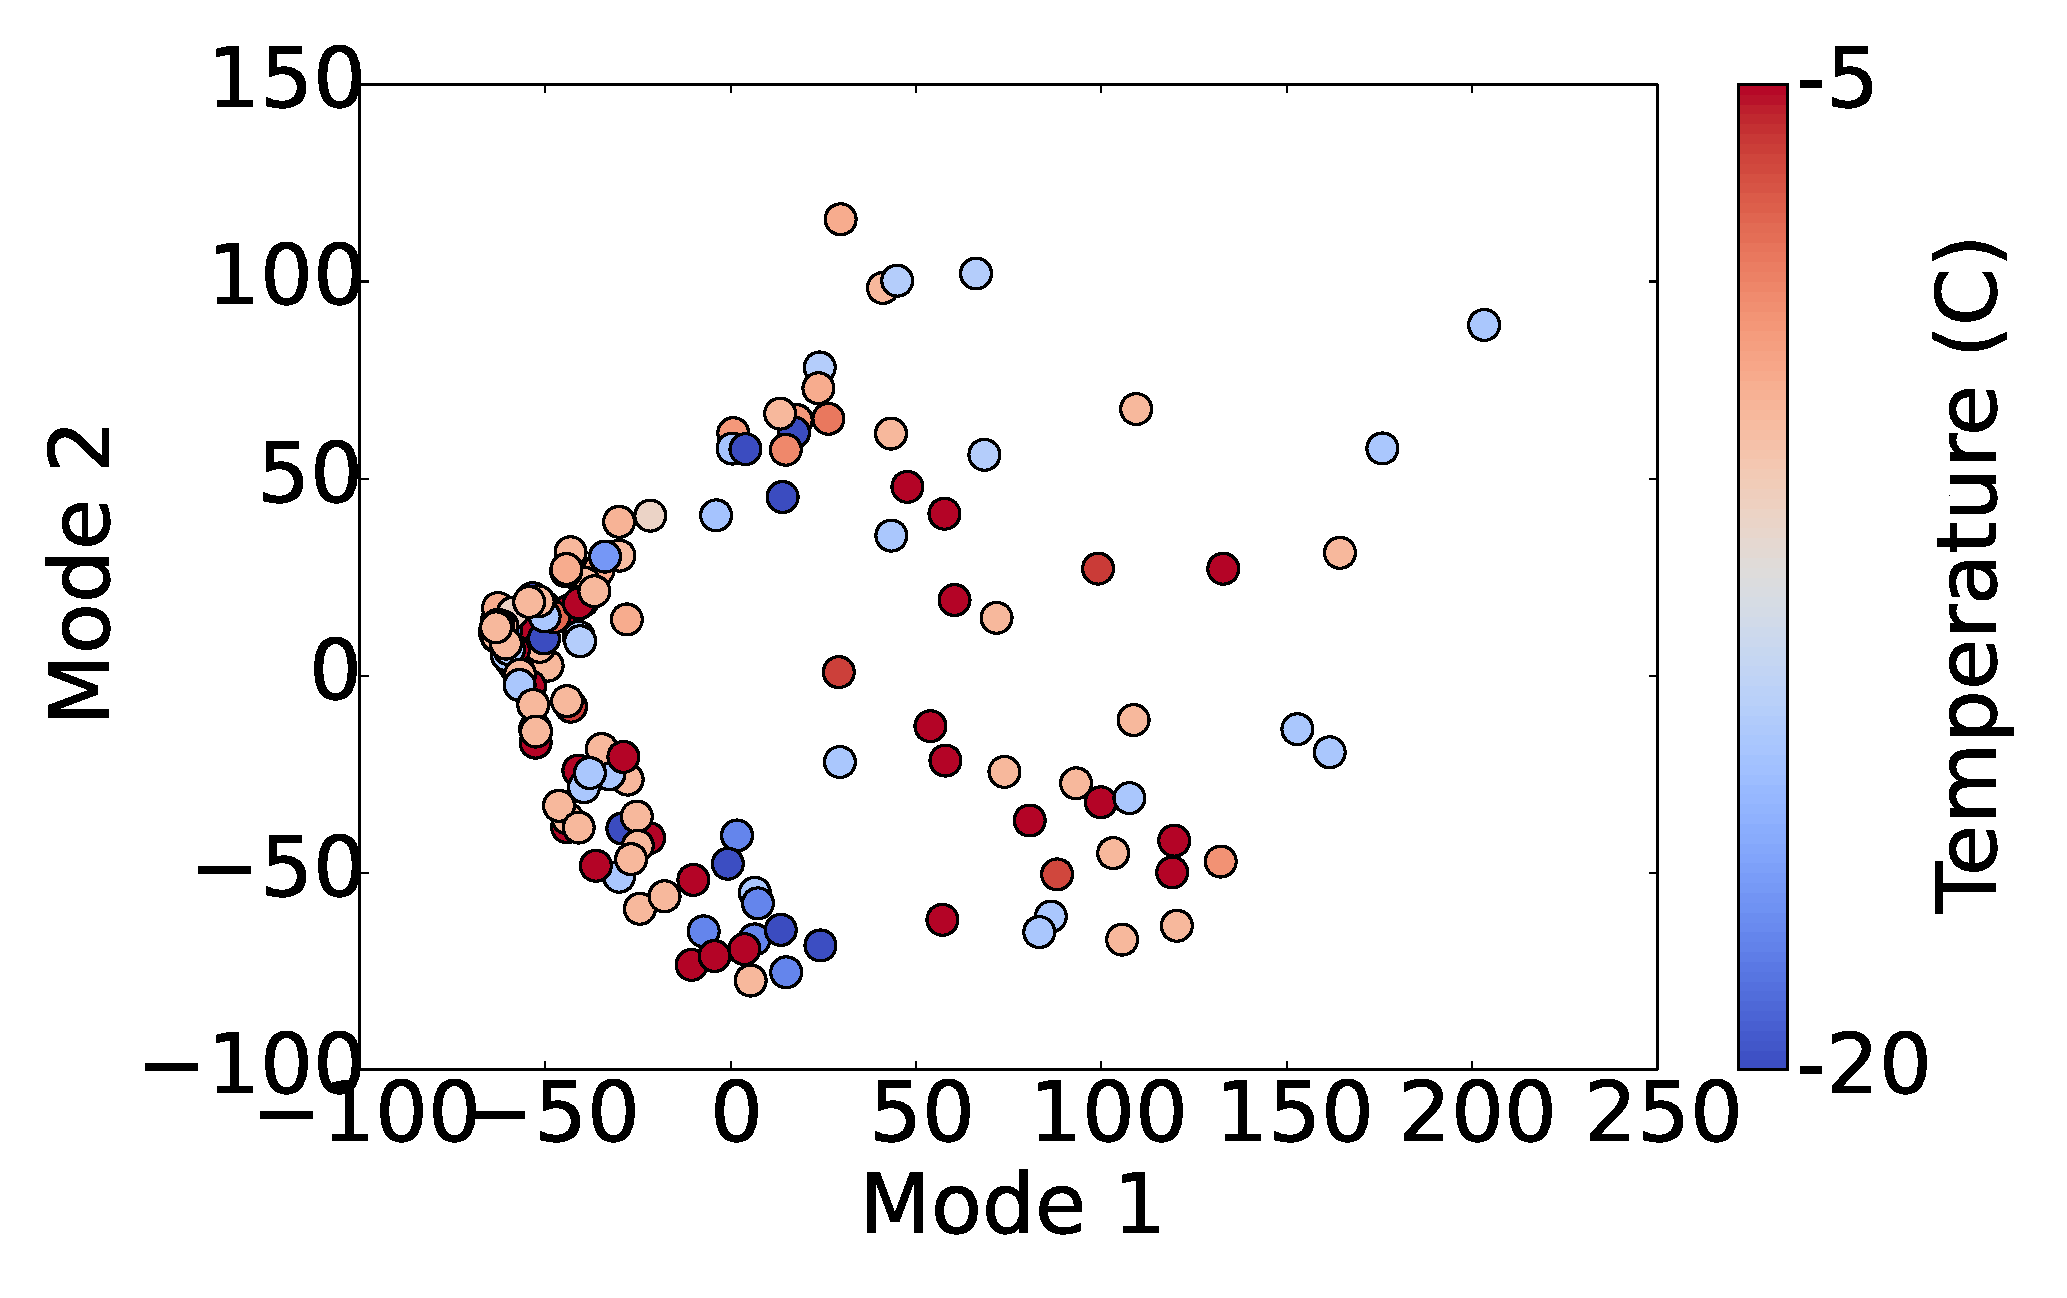
\includegraphics[width=0.4\textwidth]{10ParamMode1Mode2Temp}}
      \vspace*{-0.4cm}\subfigure{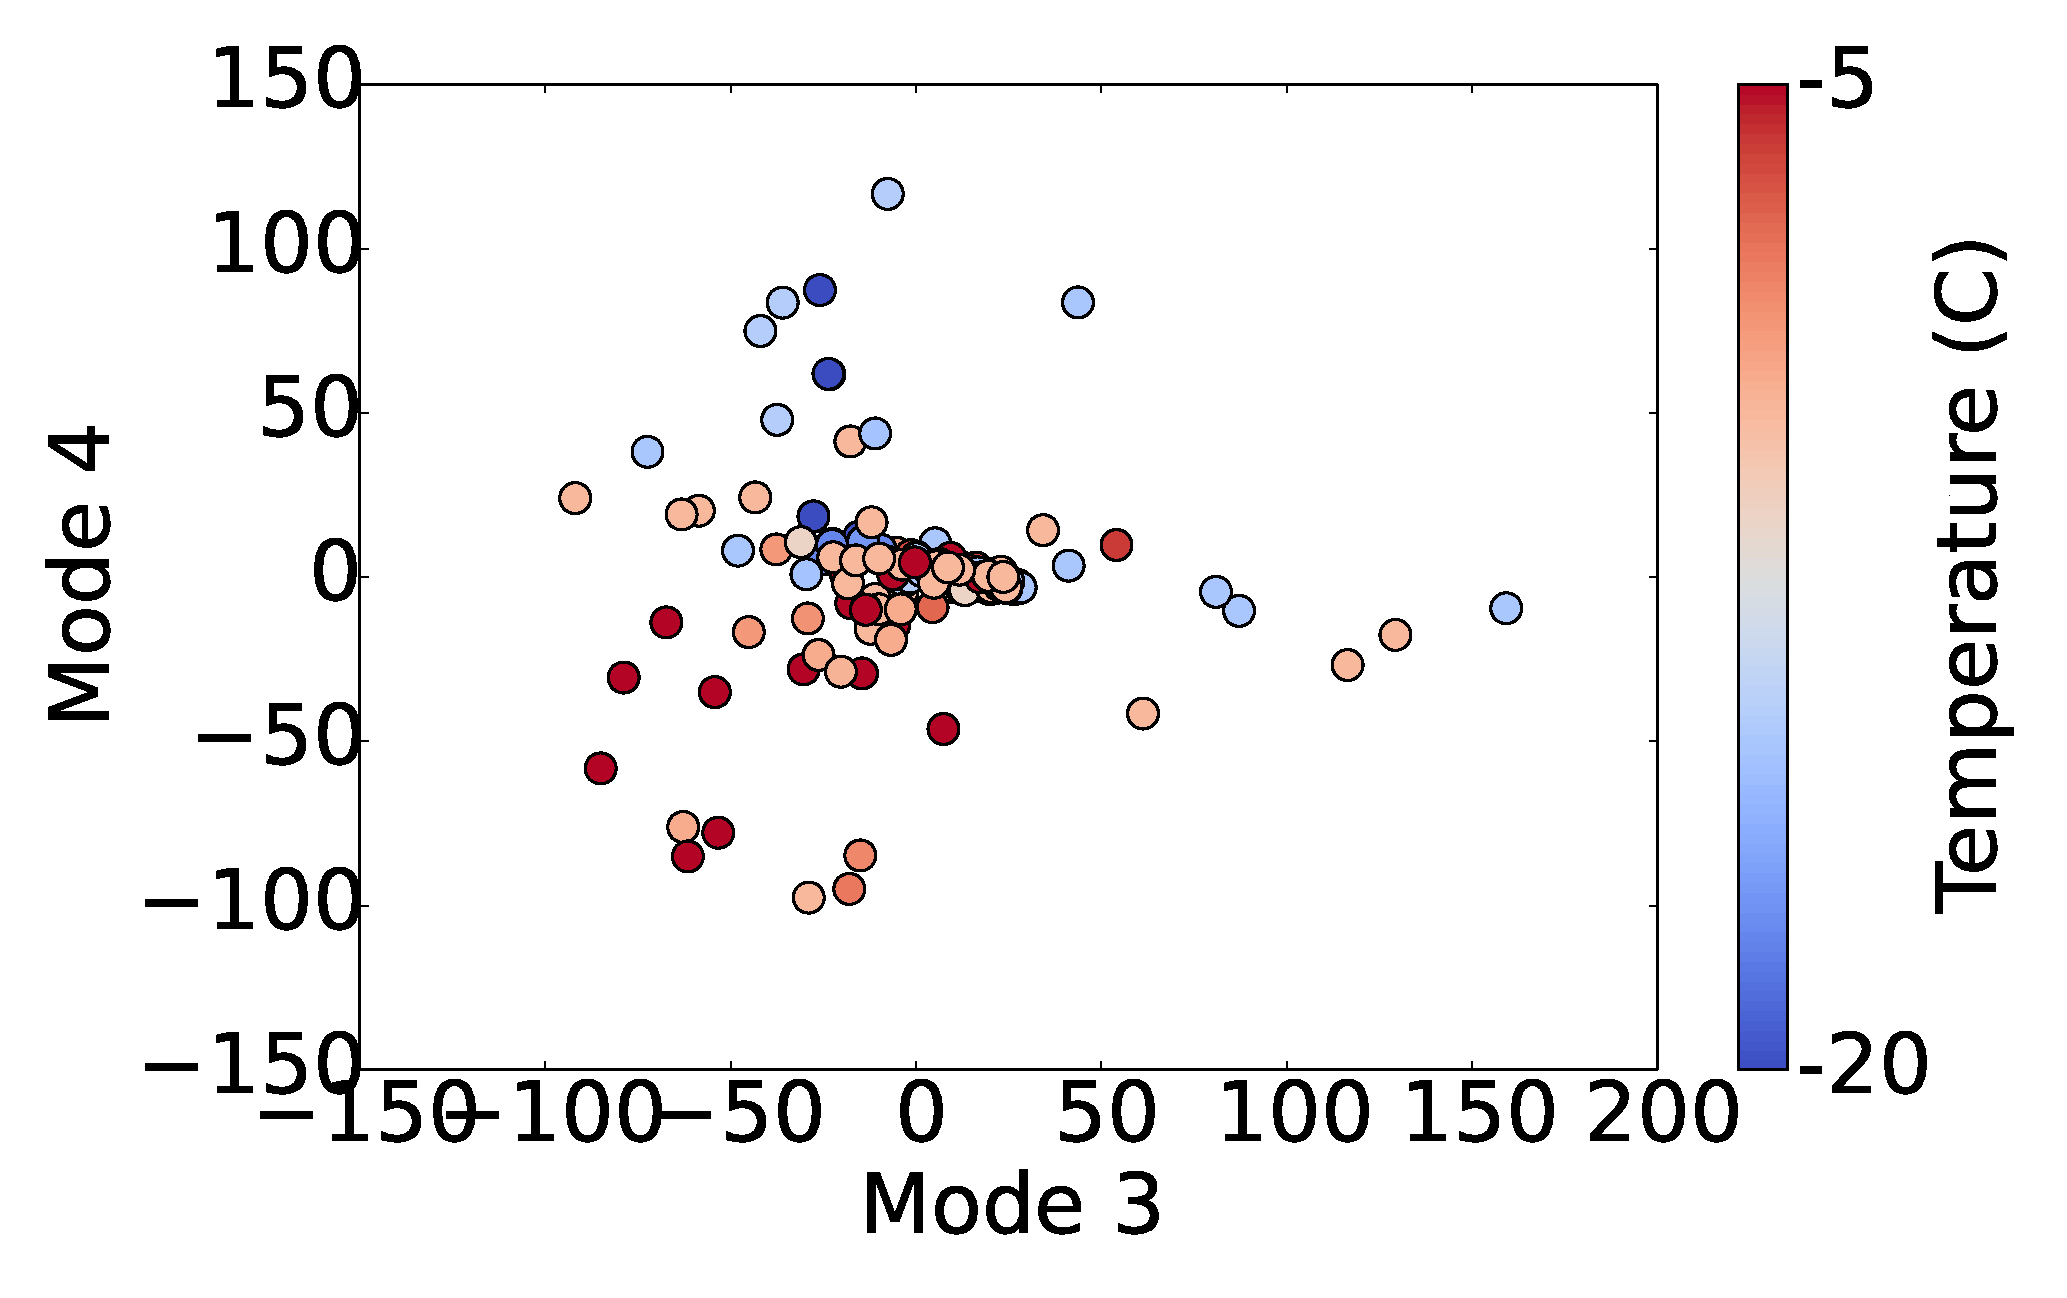
\includegraphics[width=0.4\textwidth]{10ParamMode3Mode4Temp}} \\
      \vspace*{-0.4cm}\subfigure{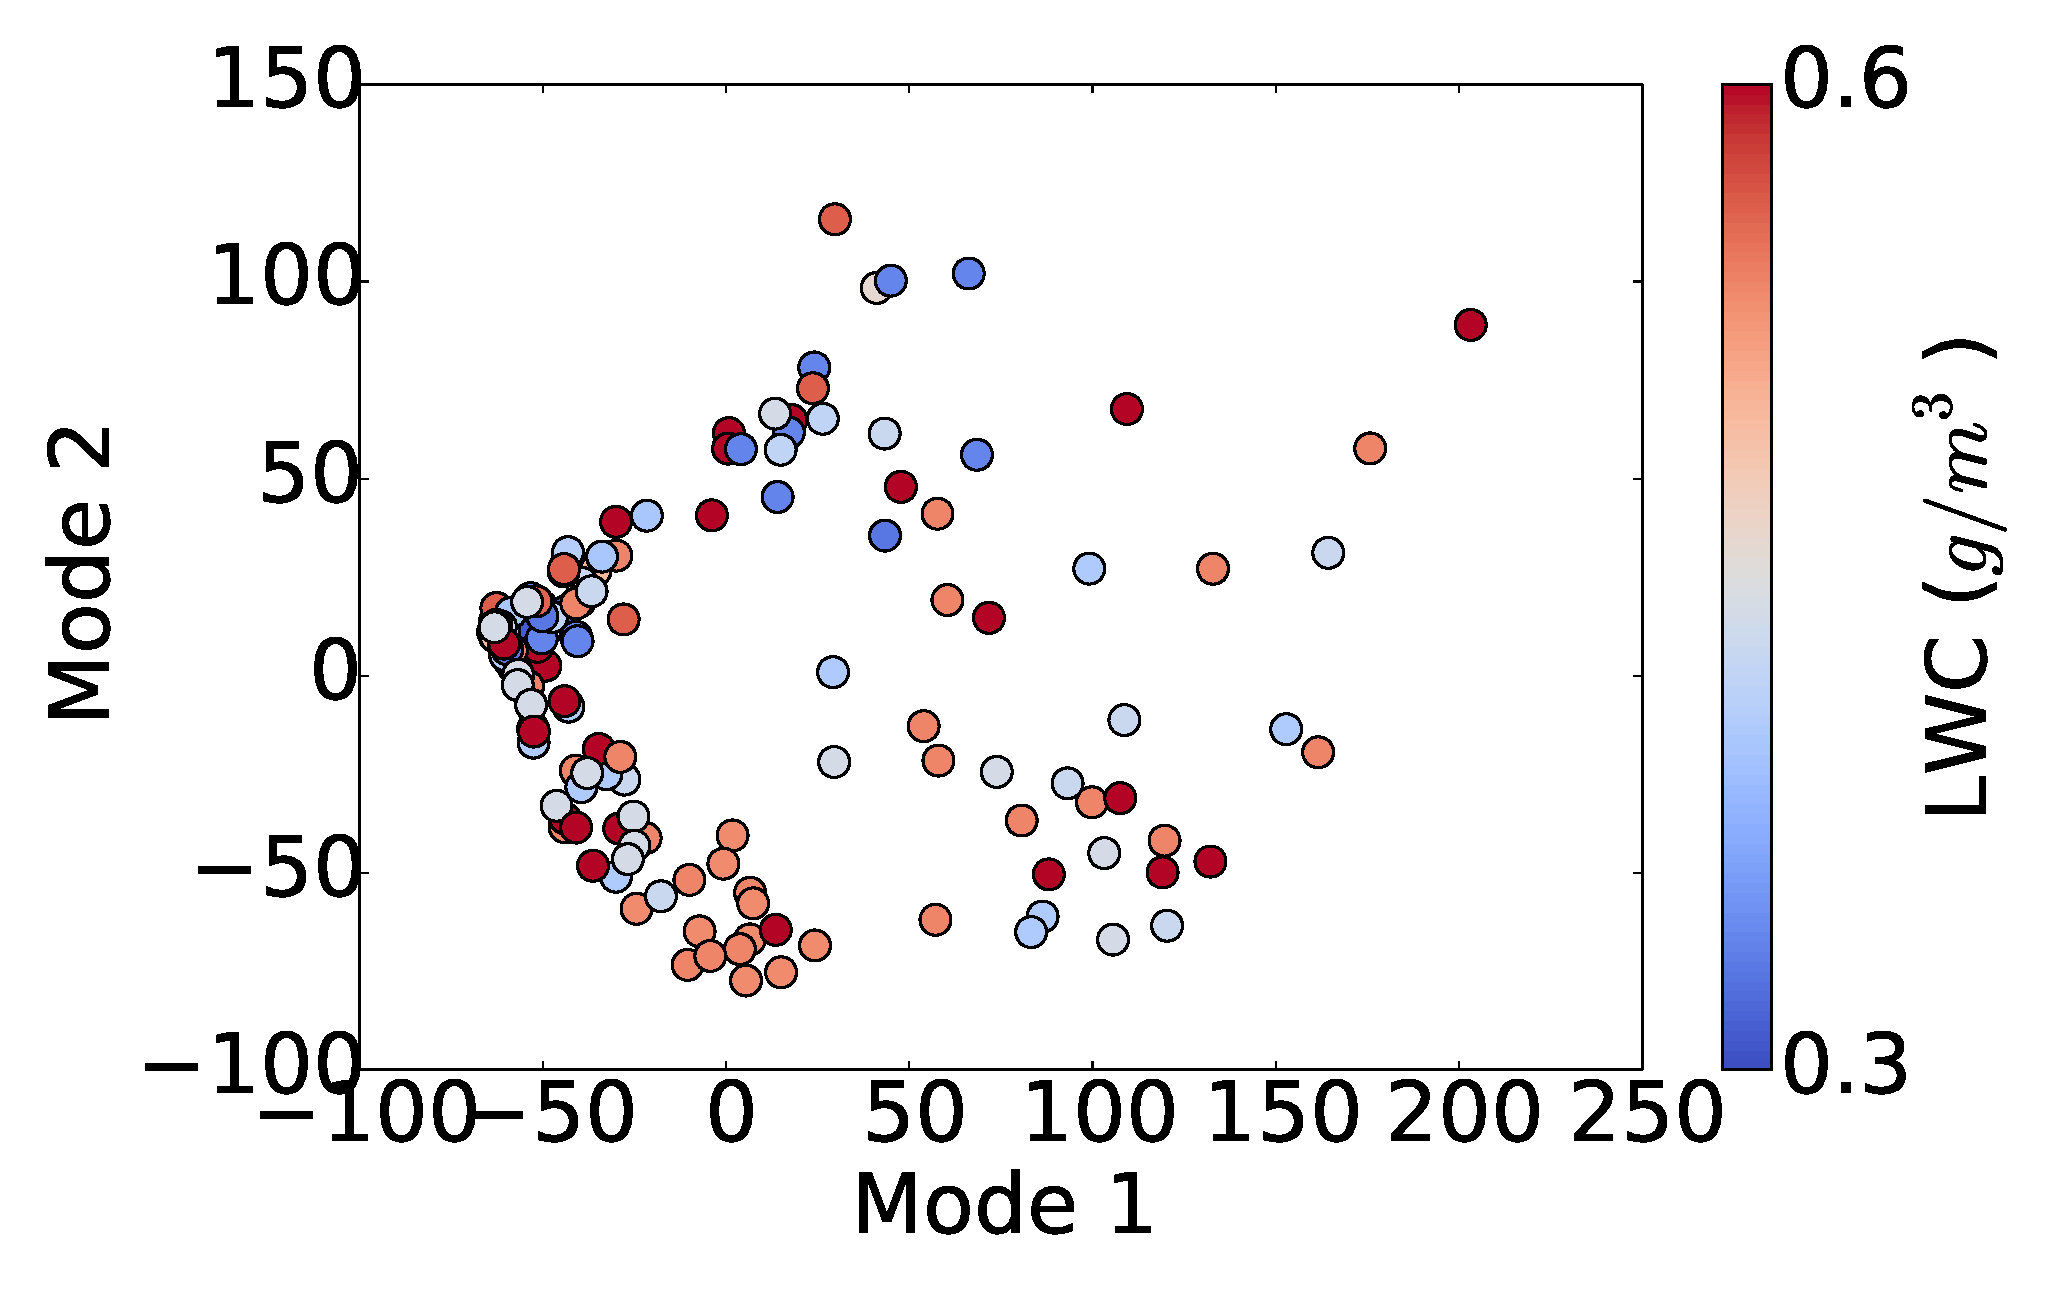
\includegraphics[width=0.4\textwidth]{10ParamMode1Mode2LWC}}
      \vspace*{-0.4cm}\subfigure{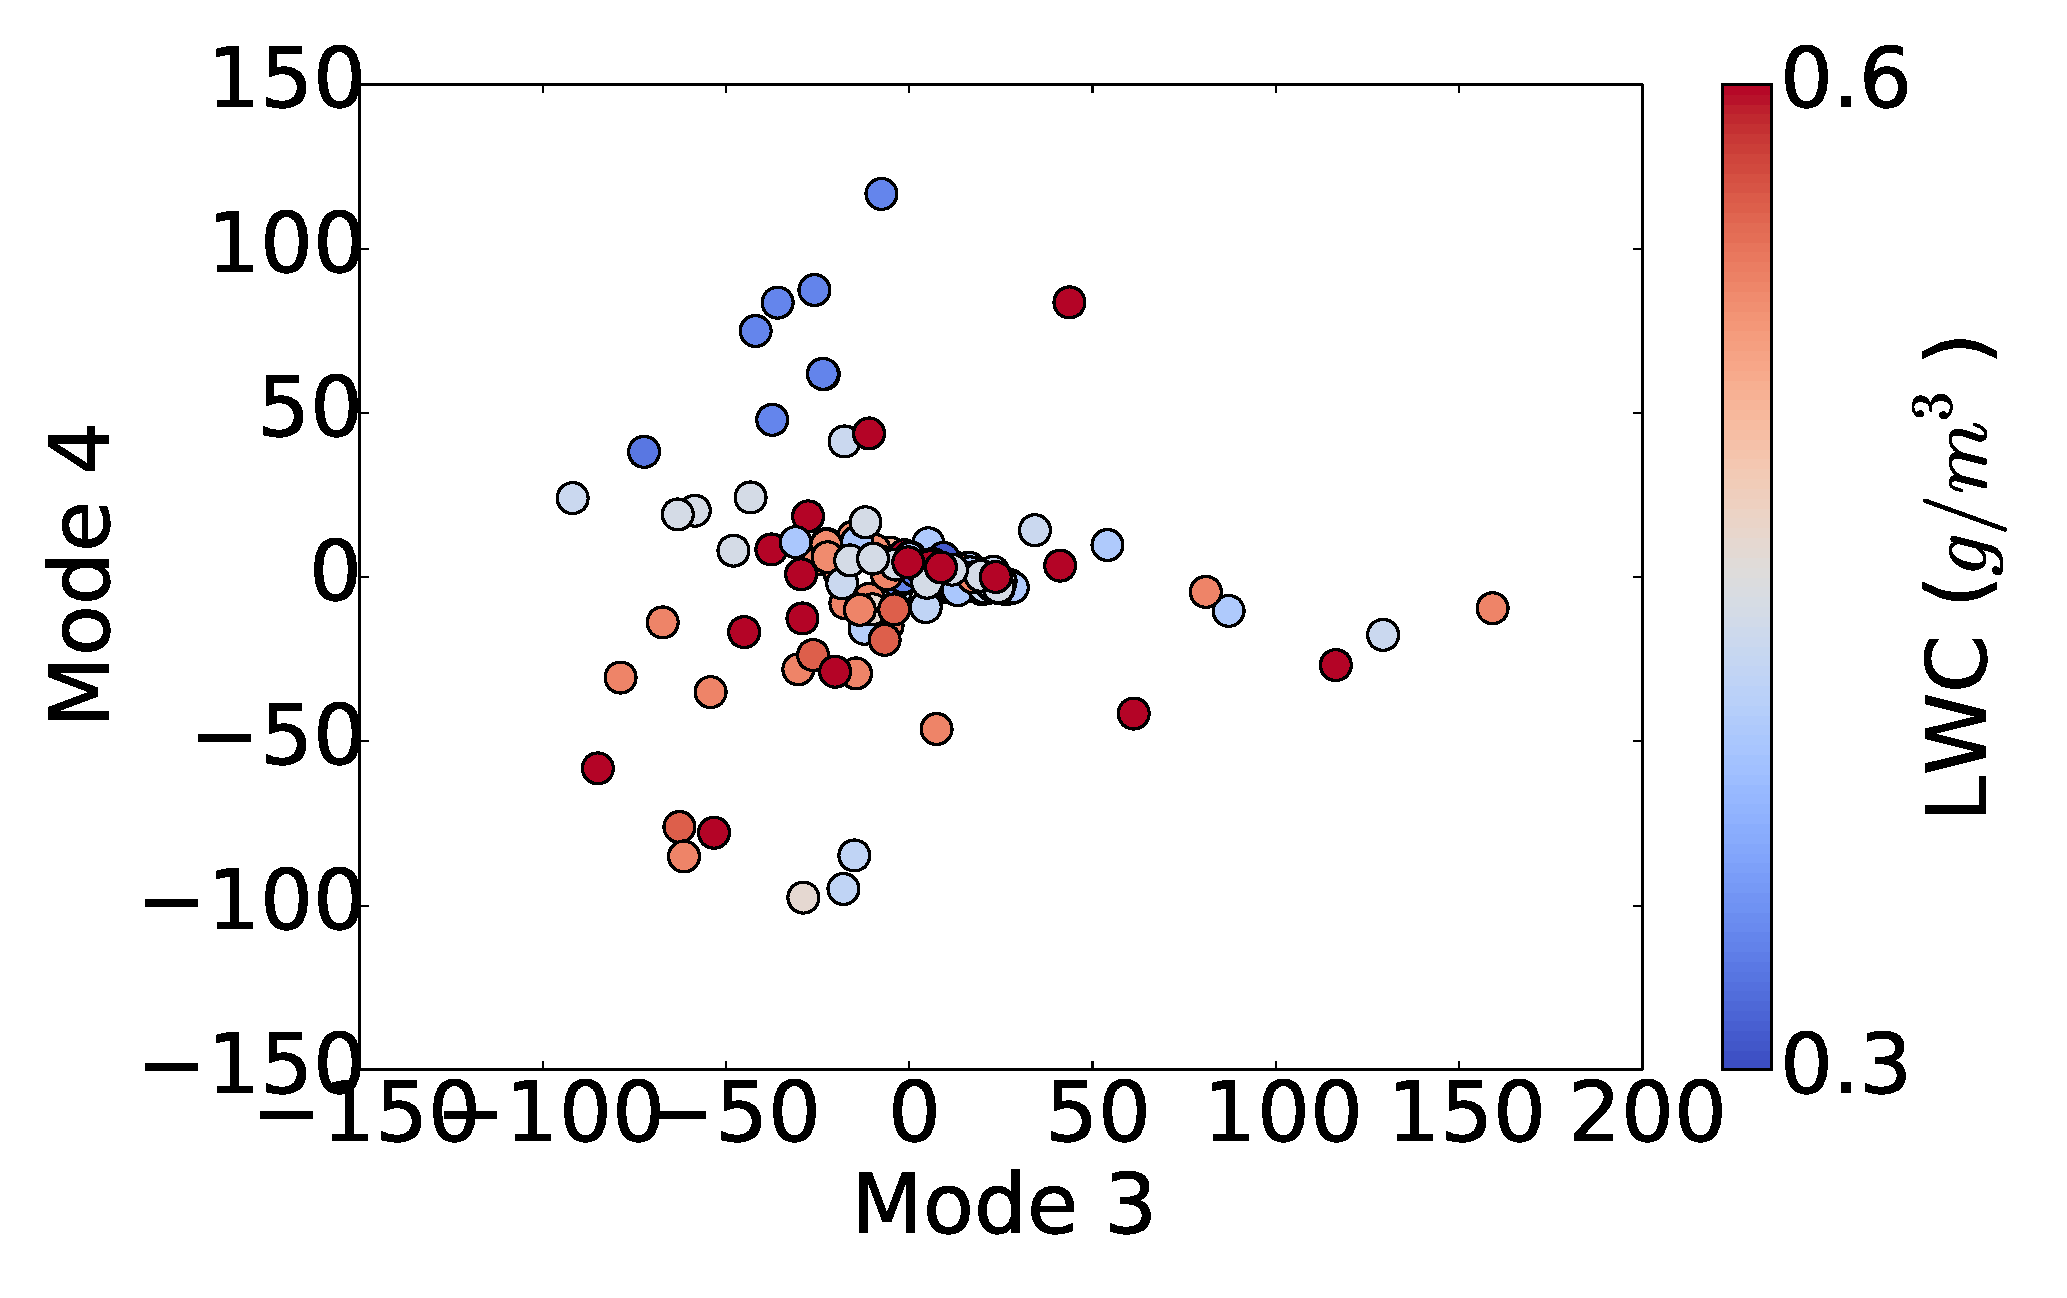
\includegraphics[width=0.4\textwidth]{10ParamMode3Mode4LWC}}
      \vspace*{0cm}\caption{POD coefficients, colored with parameters.}
\end{figure}
\end{frame}
\begin{frame}
\frametitle{Random Shapes}
\label{sec-2-7}

\begin{figure}
      \vspace*{-0.4cm}\subfigure{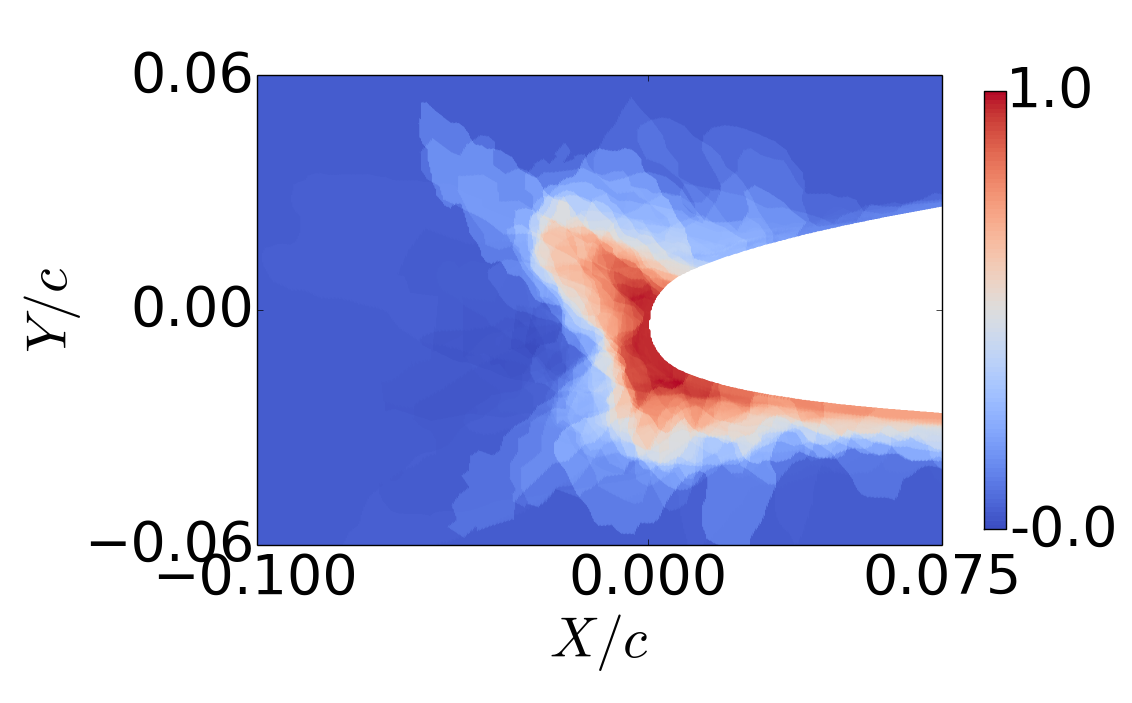
\includegraphics[width=0.4\textwidth]{10ParamHornFromPhysics}}
      \vspace*{-0.4cm}\subfigure{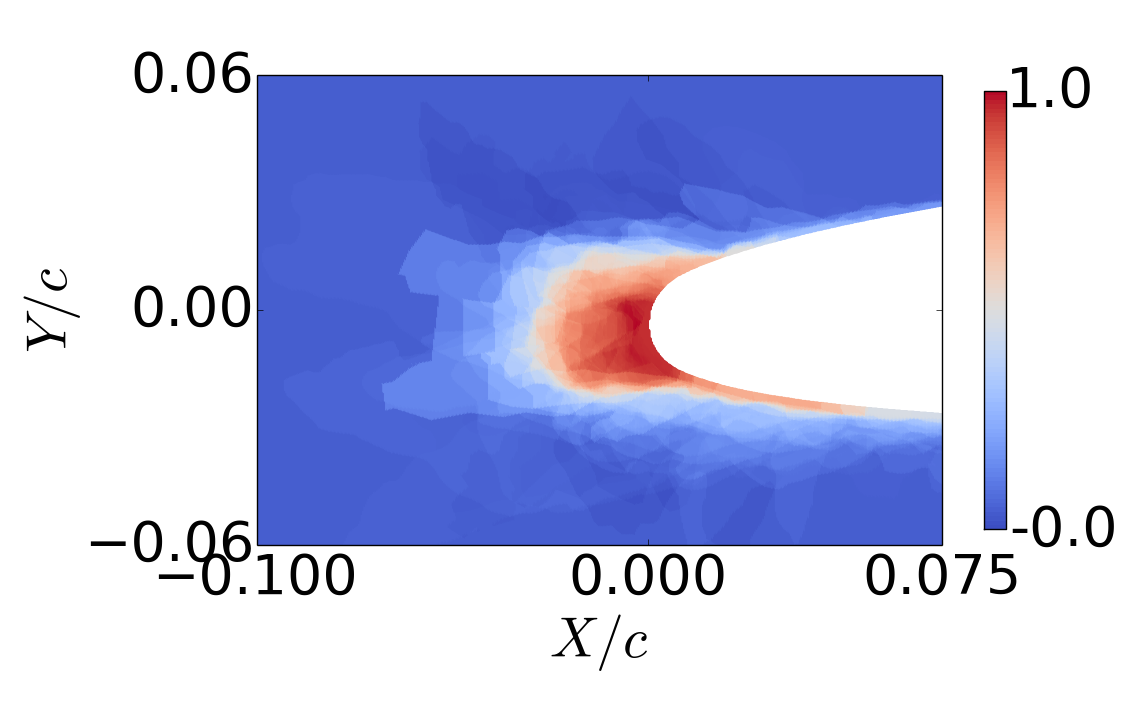
\includegraphics[width=0.4\textwidth]{10ParamRimeFromPhysics}} \\
      \vspace*{-0.4cm}\subfigure{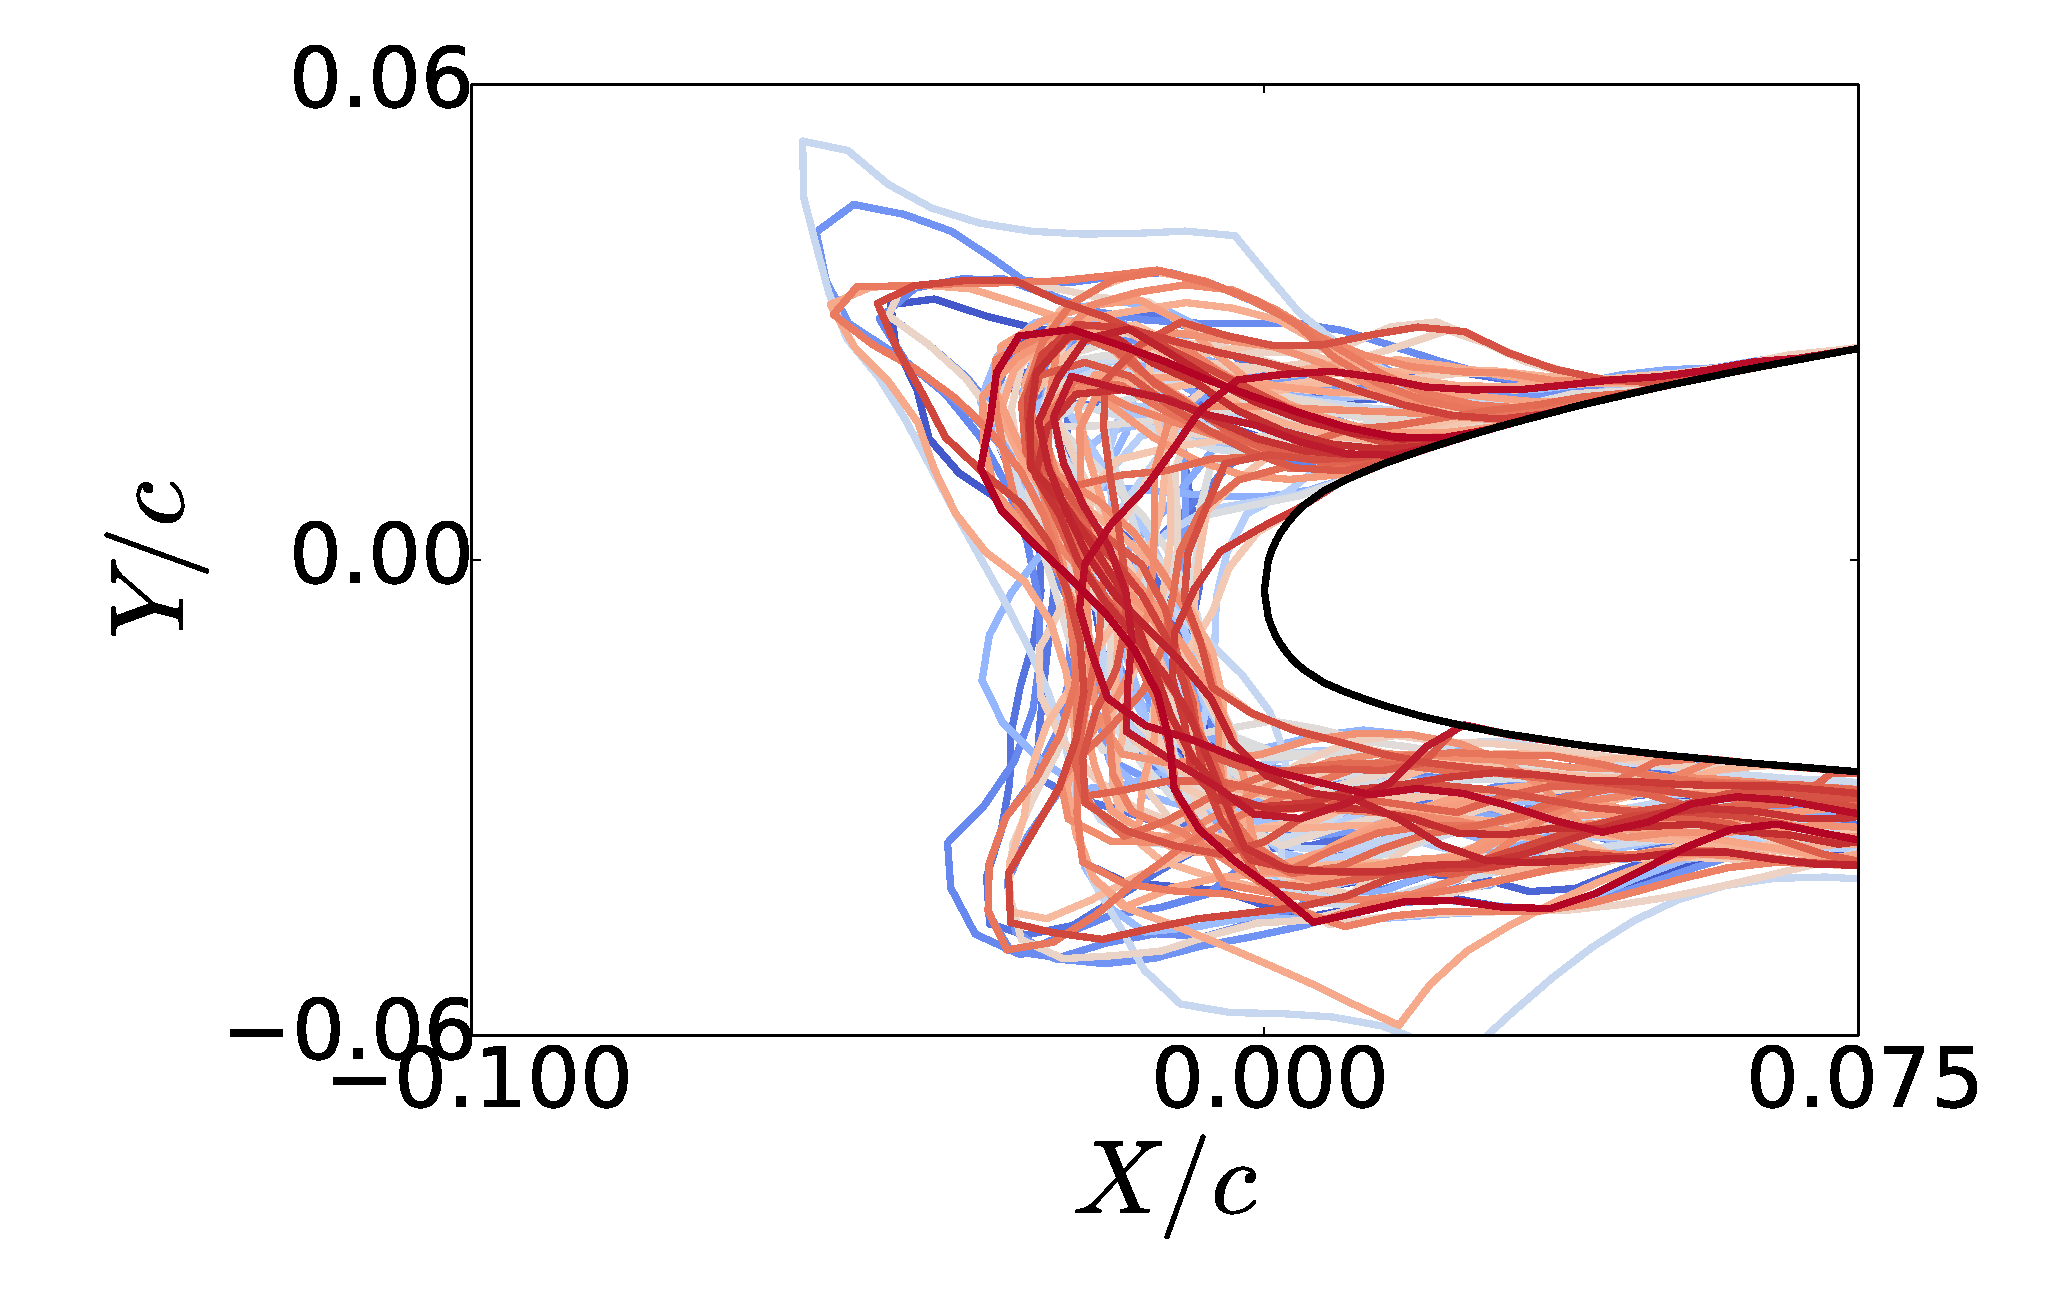
\includegraphics[width=0.4\textwidth]{10ParamRandomHorns}}
      \vspace*{-0.4cm}\subfigure{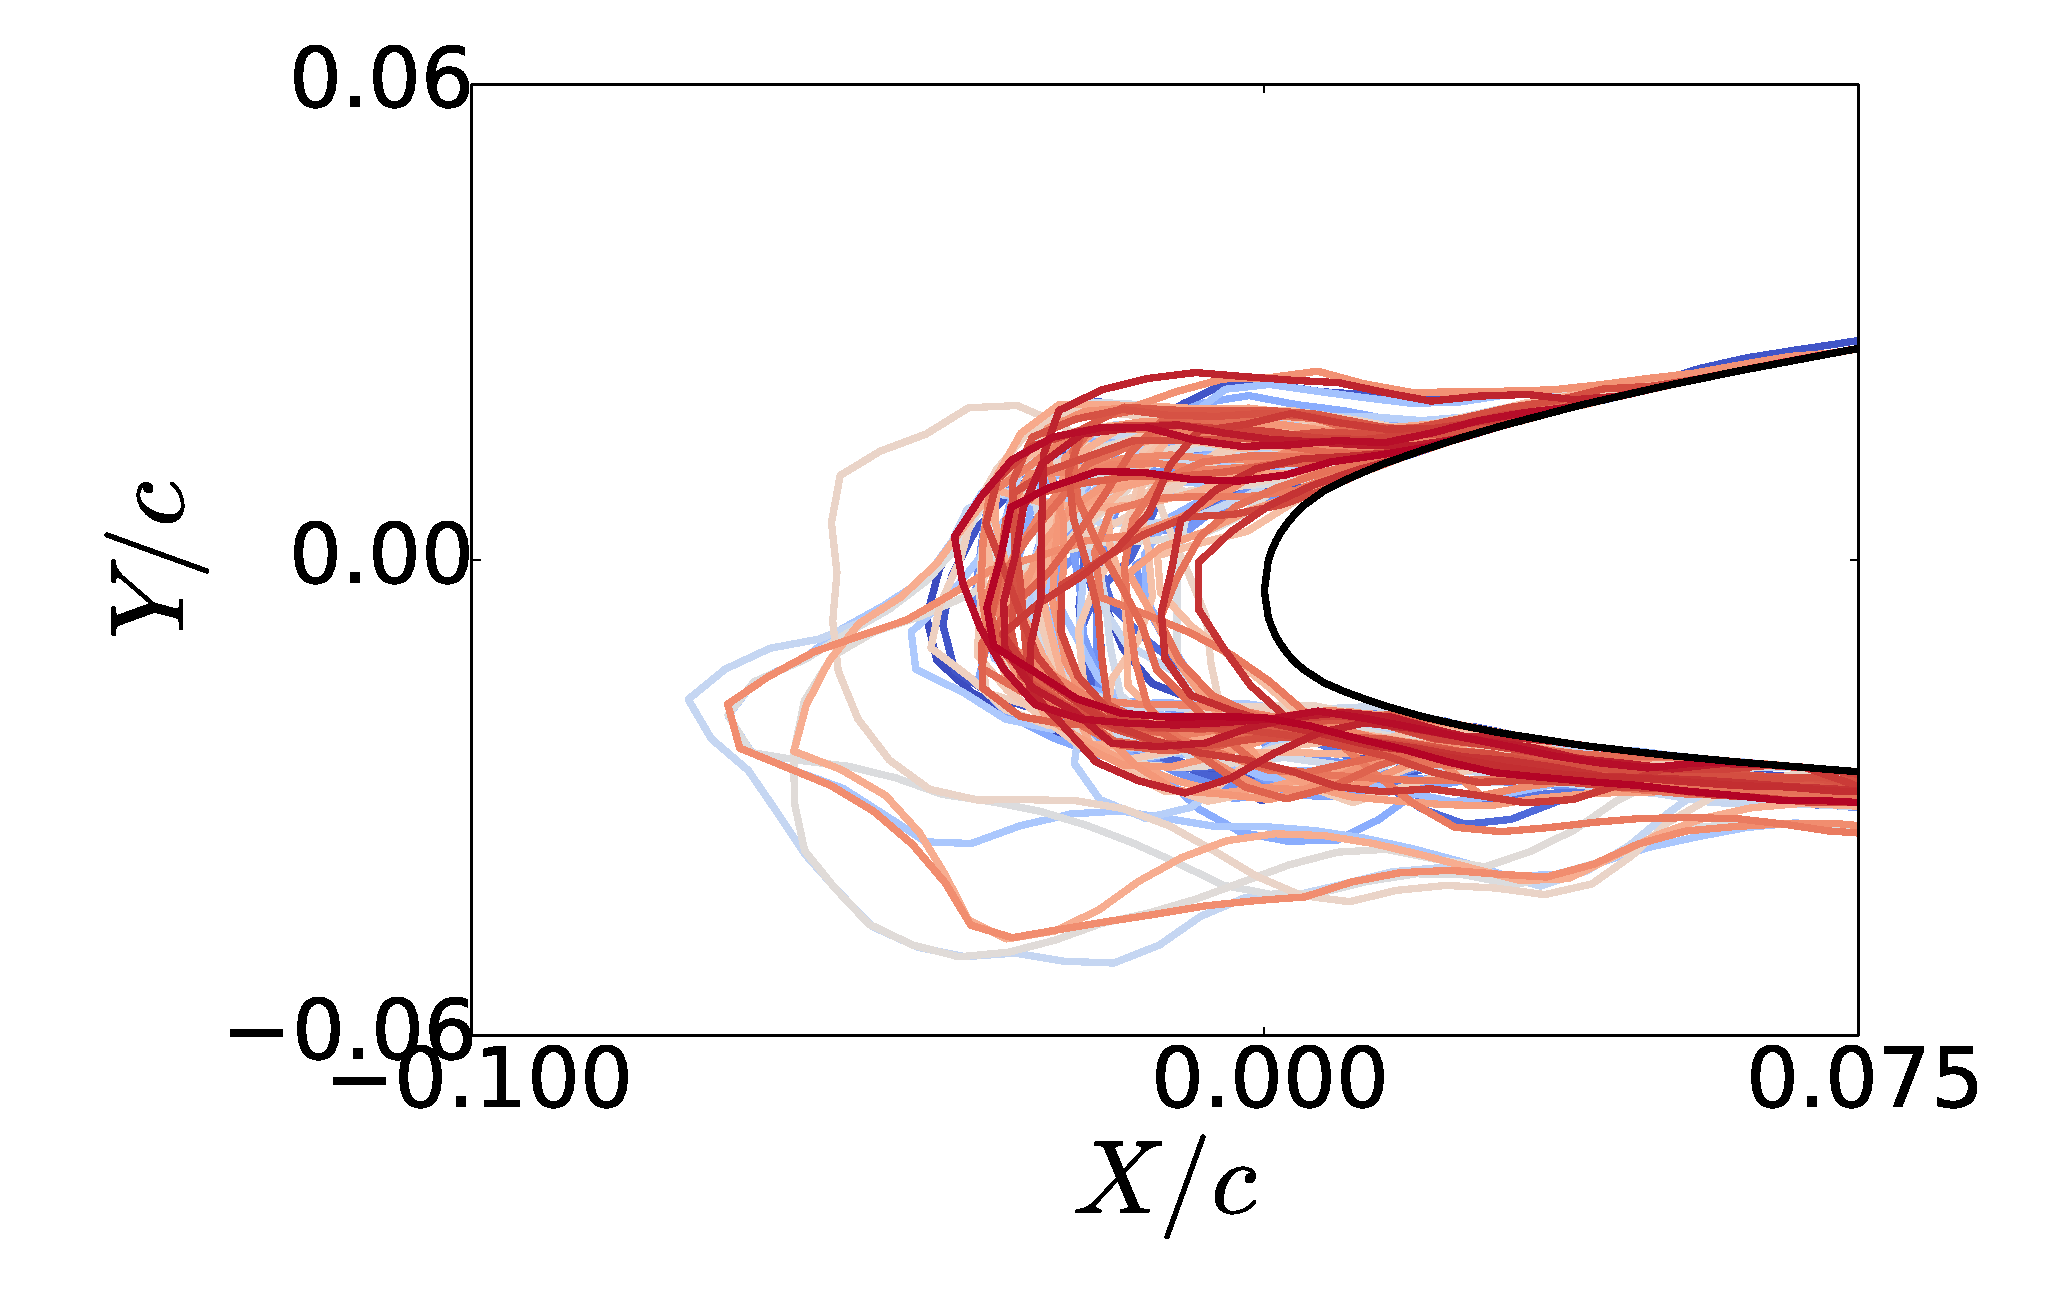
\includegraphics[width=0.4\textwidth]{10ParamRandomRime}}
      \vspace*{0cm}\caption{Random data-driven ice shapes.}
\end{figure}
\end{frame}
\begin{frame}
\frametitle{Uncertainty Quantification}
\label{sec-2-8}

\vspace*{-0.0cm}\begin{figure}
      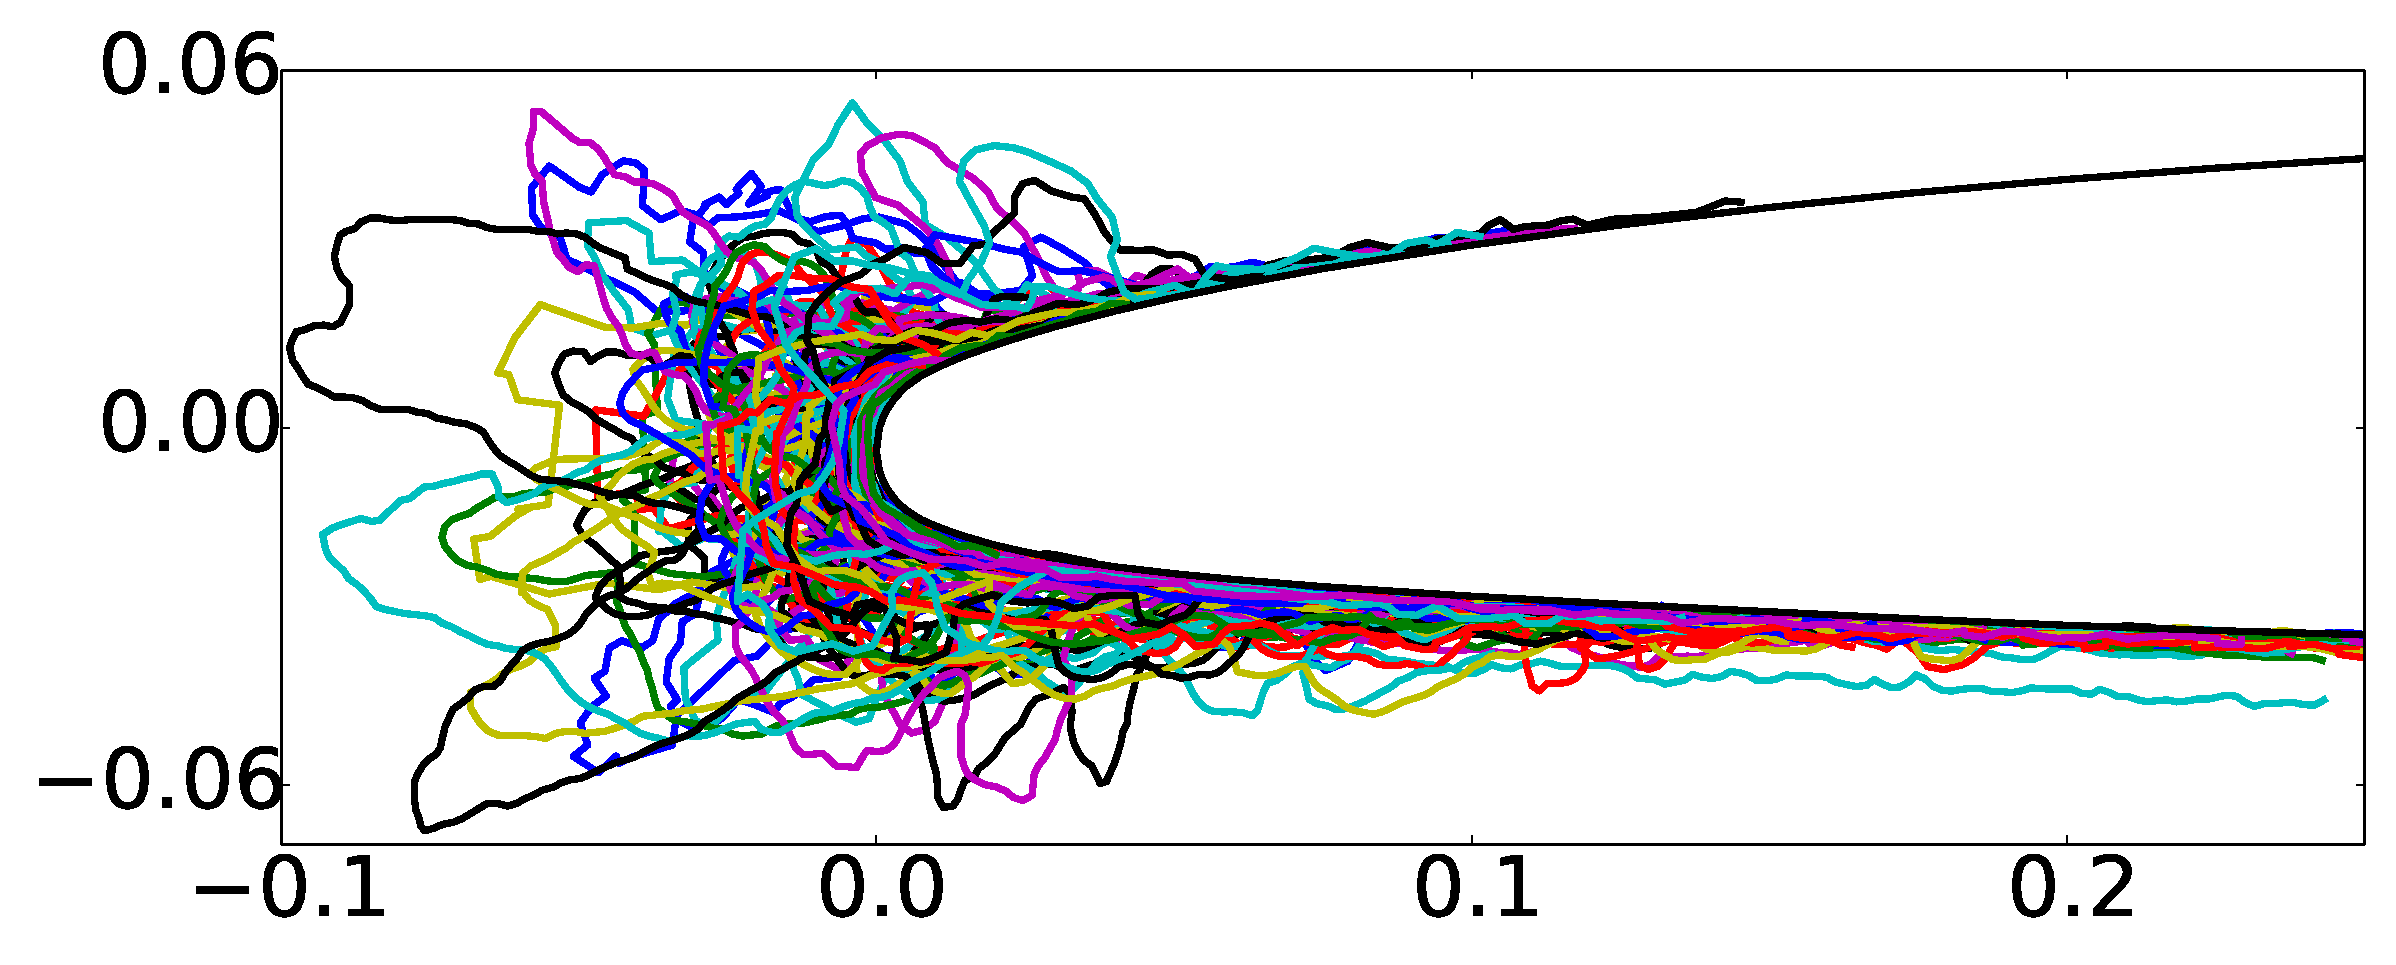
\includegraphics[width=0.5\textwidth]{GlobalDataSet}
      \caption{Wind tunnel experimental ice shapes}
\end{figure}
\textbf{Goal:} Quantify performance variation with POD modes

\textbf{Approach:}
\begin{itemize}
\item Generate random samples in POD space with Latin Hypercube Sampling (LHS)
\item Test corresponding shapes with flow solver
\item Quantify lift/drag statistics
\end{itemize}
\end{frame}
\begin{frame}
\frametitle{Latin Hypercube Samples}
\label{sec-2-9}
\end{frame}
\begin{frame}
\frametitle{Ice Shapes}
\label{sec-2-10}
\end{frame}
\begin{frame}
\frametitle{Output Statistics}
\label{sec-2-11}
\end{frame}
\begin{frame}
\frametitle{Output Statistics}
\label{sec-2-12}
\end{frame}
\section{Computational UQ}
\label{sec-3}
\begin{frame}
\frametitle{Motivation}
\label{sec-3-1}

\textbf{Investigate uncertainty in the physical process of icing}
\begin{itemize}
\item What is the statistical effect of uncertainty in physical parameters?
\begin{itemize}
\item Free-stream temperature
\item Angle of attack
\item Convective heat transfer
\item Droplet diameter distribution
\item Accretion time
\end{itemize}
\item Previous two approaches show how direct perturbations of the shape
    affect the aerodynamics
\item This approach shows how perturbations of the physics affect shape
    (and aerodynamics)
\end{itemize}
\end{frame}
\begin{frame}
\frametitle{Airfoil Icing Code Flowchart}
\label{sec-3-2}

\fontsize{7}\selectfont
% Define the layers to draw the diagram
\pgfdeclarelayer{background}
\pgfdeclarelayer{foreground}
\pgfsetlayers{background,main,foreground}

% Define block styles used later

\tikzstyle{sensor}=[draw, fill=blue!20, text width=5em, 
    text centered, minimum height=2.5em,drop shadow]
\tikzstyle{ann} = [above, text width=5em, text centered]
\tikzstyle{wa} = [sensor, text width=7.5em, fill=blue!20, 
    minimum height=3em, rounded corners, drop shadow]

% Define distances for bordering
\def\blockdist{2.3}
\def\edgedist{2.5}

\begin{tikzpicture}
    \node (CleanAirfoil) [wa]  {Clean Airfoil Geometry};
    \path (CleanAirfoil)+(4,2.5) node (FlowSolver) [wa] {Mesh/Flow Solver};
    \path (FlowSolver)+(0,-1.25) node (Droplet) [wa] {Droplet\\Advection Module};
    \path (Droplet)+(0,-1.25) node (ThermoModule) [wa] {Thermodynamic Module};
    \path (ThermoModule)+(0,-1.25) node (IcedAirfoil) [wa] {Iced Airfoil Geometry};
    \path (CleanAirfoil)+(8,0) node (FinalAirfoil) [wa] {Final Iced Airfoil Geometry};

    \path [draw, ->, thick] (CleanAirfoil.north) |- node [above] {} (FlowSolver.west);
    \path [draw, ->, thick] (FlowSolver.south) -- node [below] {} (Droplet.north);
    \path [draw, ->, thick] (Droplet.south) -- node [below] {} (ThermoModule.north);
    \path [draw, ->, thick] (ThermoModule.south) -- node [below] {} (IcedAirfoil.north);
    \path [draw, ->, thick] (IcedAirfoil.east) -| node [above] {} (FinalAirfoil.south);
    \path [draw, ->, thick] (IcedAirfoil.east) -- ++(0.75,0cm) |- node [above]
                      {} (FlowSolver.east);

    \begin{pgfonlayer}{background}
        \path (FlowSolver.west)+(-1,1) node (a) {};
        \path (IcedAirfoil.east)+(1,-1) node (b) {};
        \path[fill=orange!20,rounded corners, draw=black!50, dashed] (a) rectangle (b);
            
    \end{pgfonlayer}

\end{tikzpicture}
\end{frame}
\begin{frame}
\frametitle{Droplet Advection}
\label{sec-3-3}

\textbf{Advection Equations:} \\
\begin{equation*}
  \begin{align}
    \frac{d \bv{x}}{d t} &= \bv{v} \\
    m \frac{d \bv{v}}{d t} &= \frac{1}{2} \rho_g C_D \pi r^2 ||\bv{v_g} - \bv{v}|| (\bv{v_g} - \bv{v}) + m \bv{g}
  \end{align}
\end{equation}

\begin{columns}[c]
  \column{0.5\textwidth}
    \centering
    \begin{figure}
    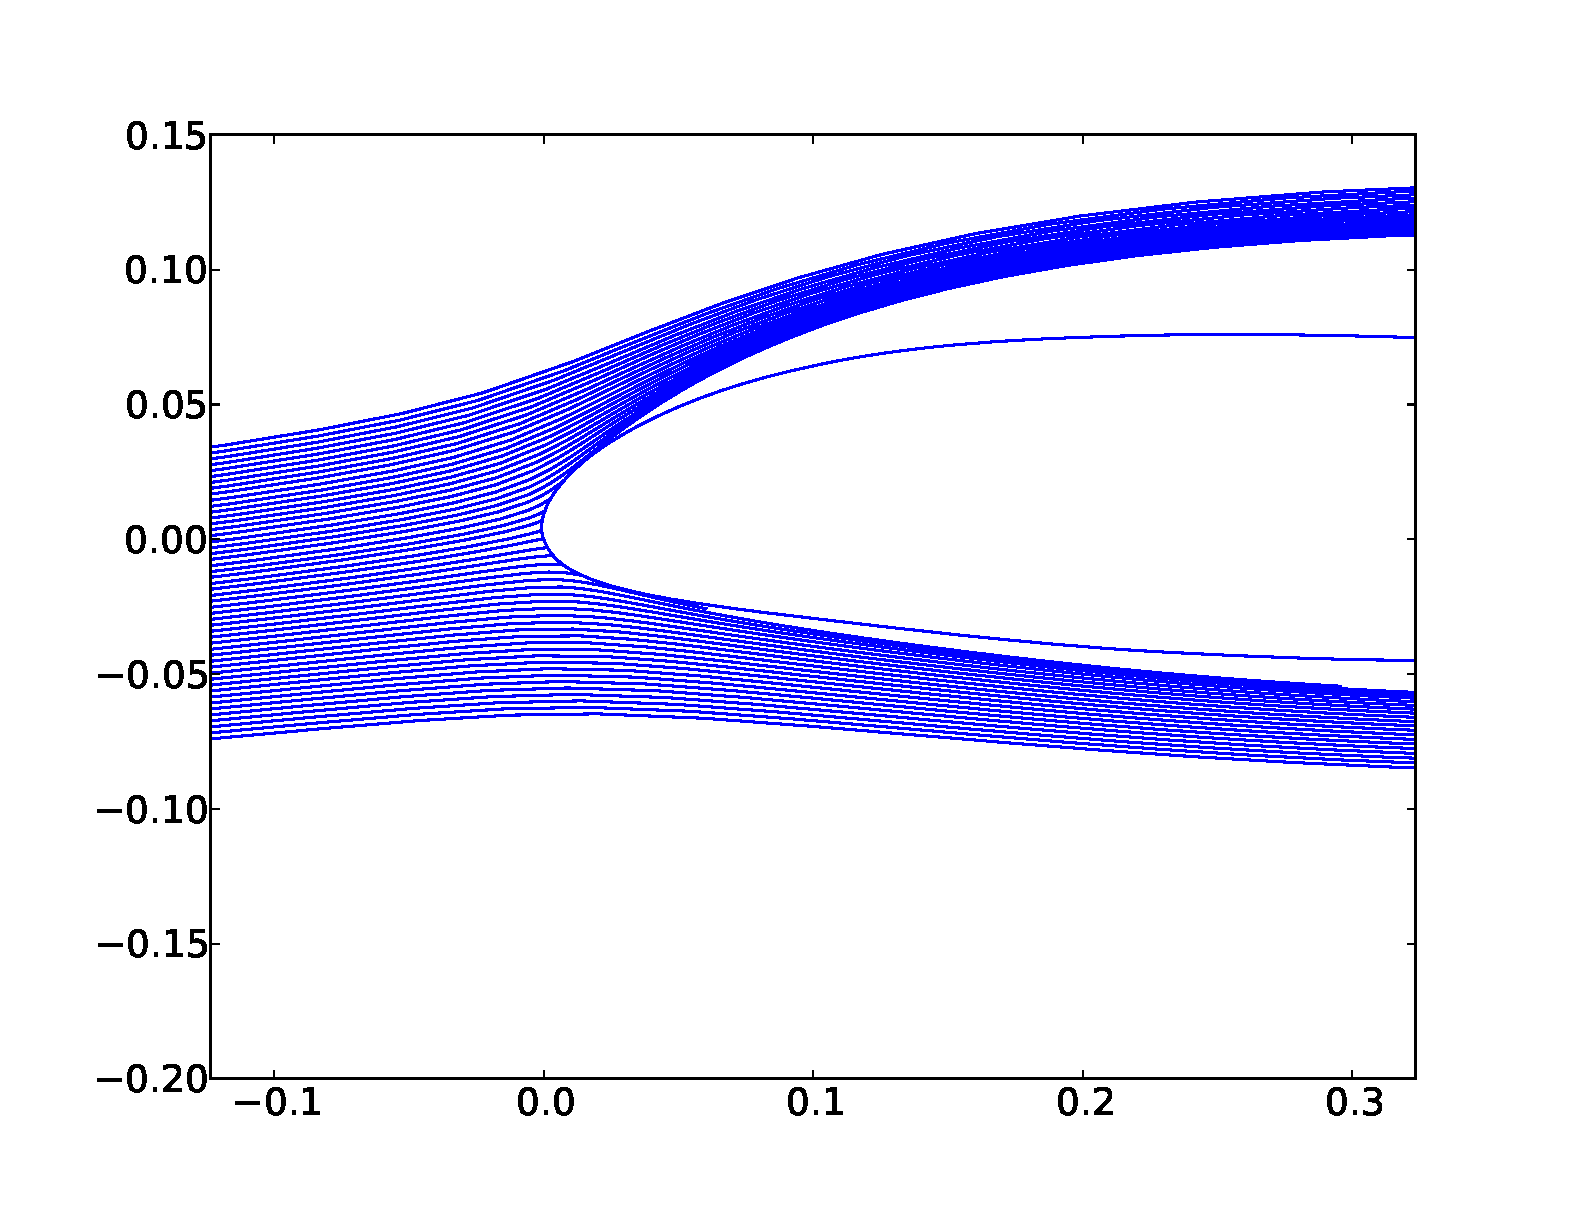
\includegraphics[width=0.9\textwidth]{ExampleR10em6}
    \caption{R = 10$\mu$m}
    \end{figure}
  \column{0.5\textwidth}
    \centering
    \begin{figure}
    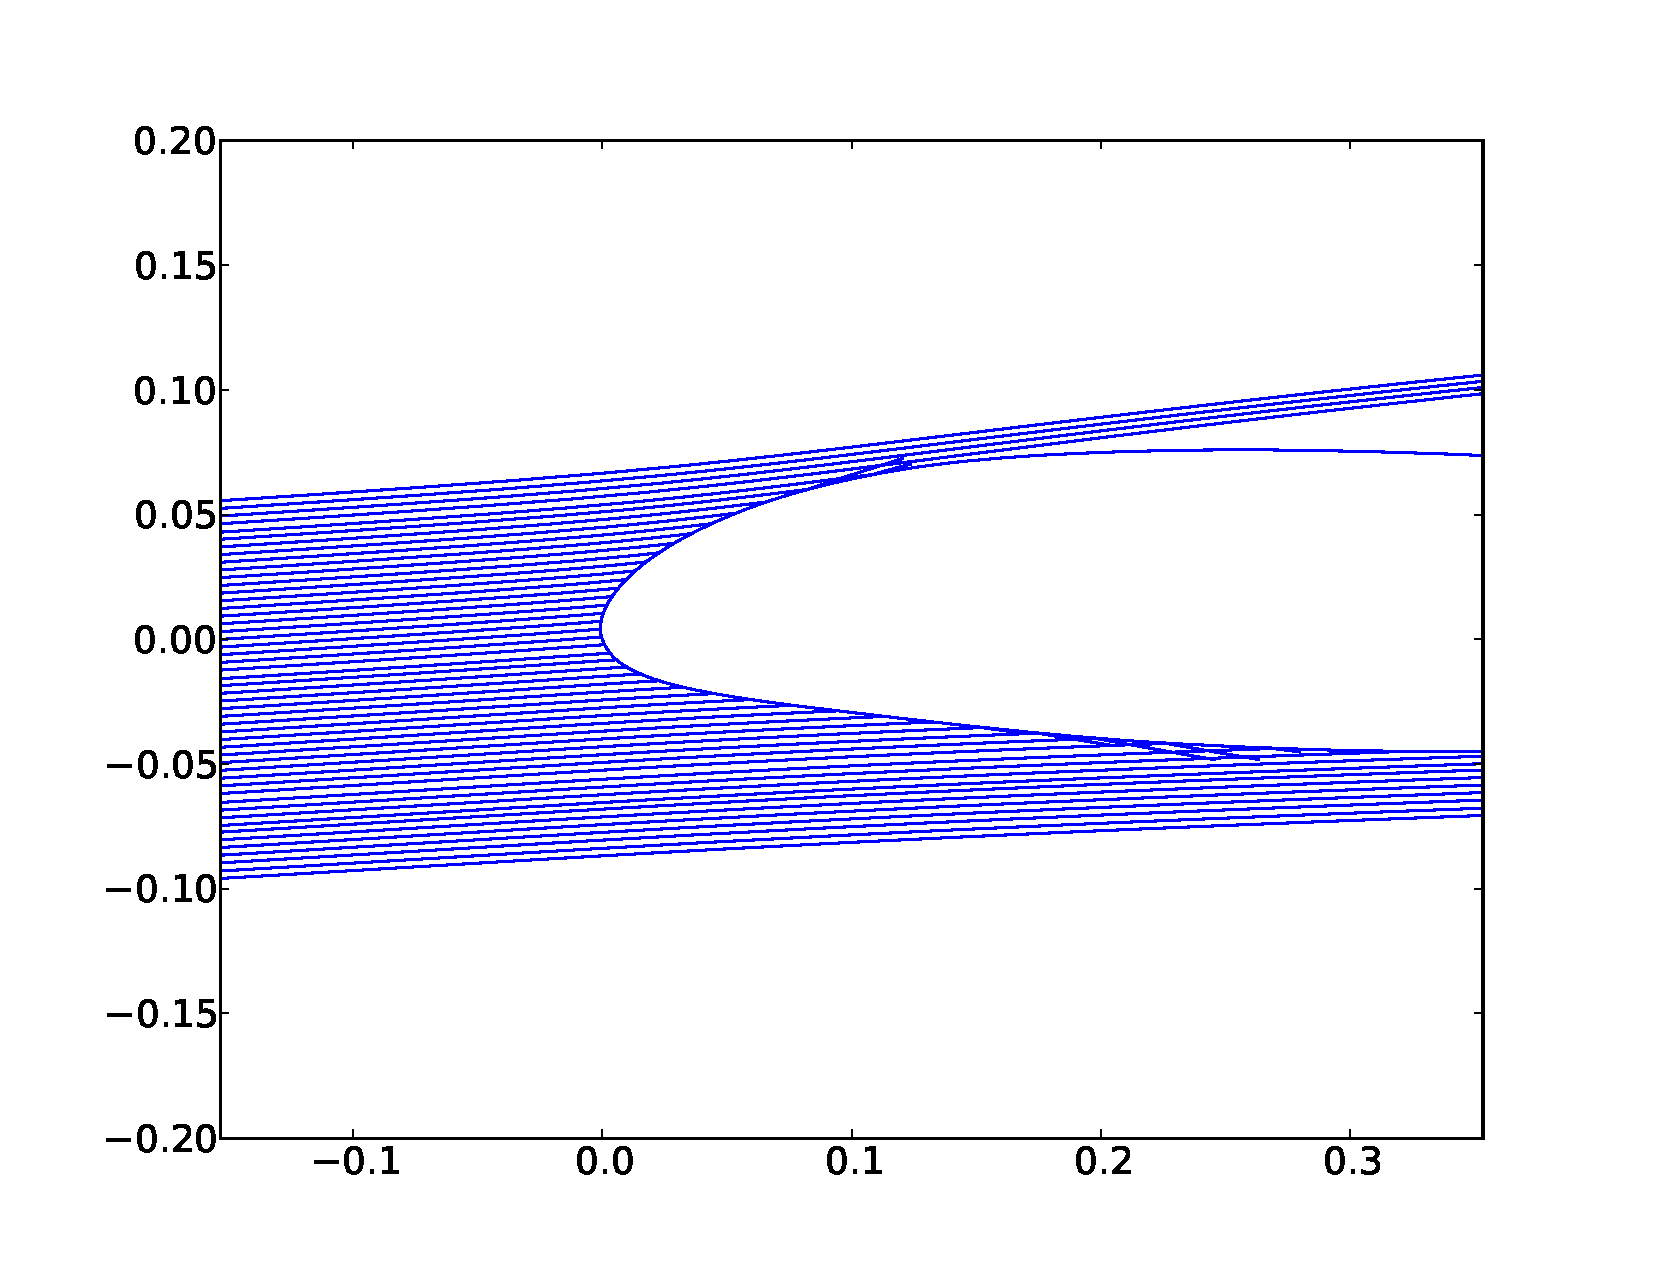
\includegraphics[width=0.9\textwidth]{ExampleR100em6} \\
    \caption{R = 100$\mu$m}
    \end{figure}
\end{columns}
\end{frame}
\begin{frame}
\frametitle{Thermodynamics}
\label{sec-3-4}

\textbf{Conservation Equations:} \\
\begin{equation*}
  \begin{align}
    \rho_w \left \lbrace \frac{\partial h_f}{\partial t} + \nabla \cdot (\bv{u_f} h_f) \right \rbrace &= \dot{m}_{imp} - \dot{m}_{evap} - \dot{m}_{ice} \\
    \rho_w \left \lbrace \frac{\partial (h_f c_W T)}{\partial t} + \nabla \cdot (\bv{u_f} h_f c_W T) \right \rbrace &= \left [ c_W T_d + \frac{u_d^2}{2} \right ] \dot{m}_{imp} \\
    & - L_{evap} \dot{m}_{evap} \\
    & +(L_{fus} + c_{ice}T)\dot{m}_{ice} \\
    & + c_H (T_{Rec} - T)
  \end{align}
\end{equation}

\begin{itemize}
\item \textbf{Mass}
\begin{itemize}
\item Enters through impinging droplets
\item Exits via evaporation/sublimation and freezing
\end{itemize}
\item \textbf{Energy}
\begin{itemize}
\item Enters through impinging droplets, freezing of ice
\item Exits via evaporation/sublimation, radiation, convection
\end{itemize}
\item Solution procedure: explicit marching, finite volume discretization
  with upwinded derivatives
\end{itemize}
\end{frame}
\begin{frame}
\frametitle{Preliminary Intermediate Results: Ice Shapes}
\label{sec-3-5}

    \centering
    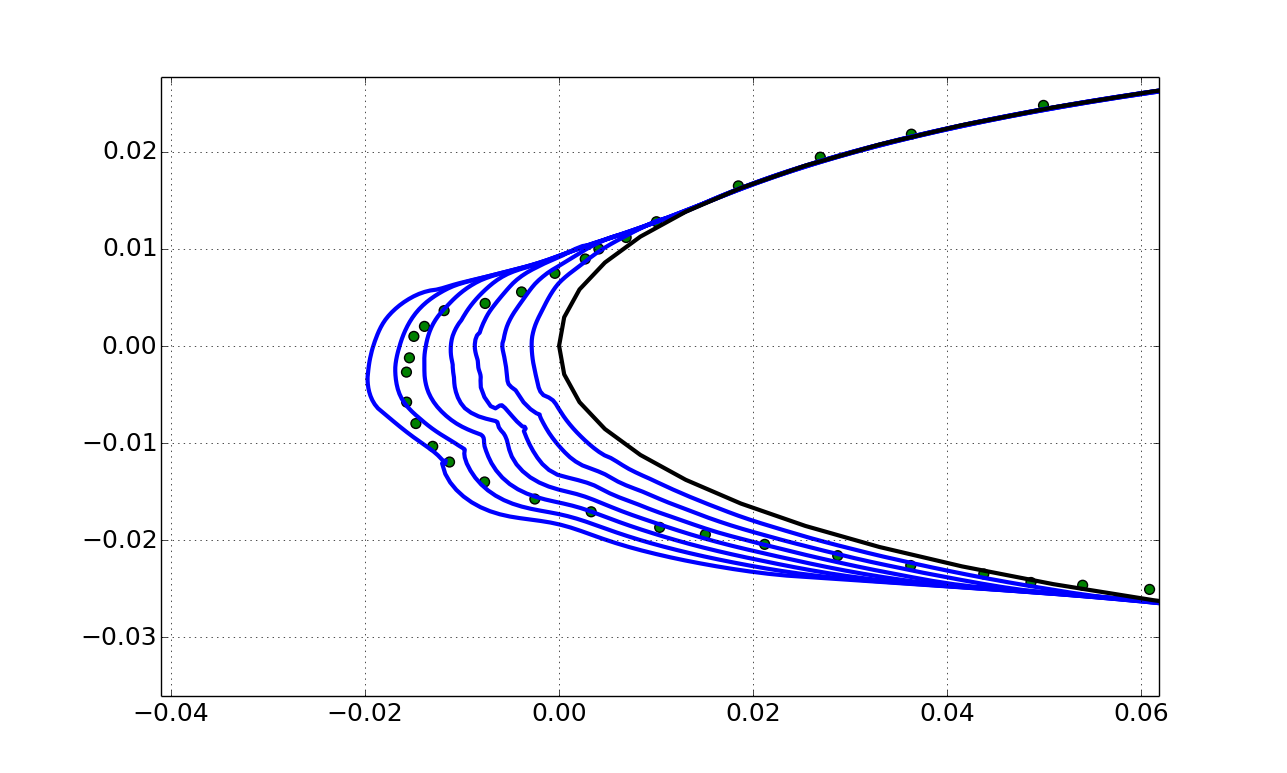
\includegraphics[width=0.65\textwidth]{Rime405Example.png}

\begin{itemize}
\item NACA0012, $\alpha = 4^o$, $T_{\infty} = 256 K$, $U_{\infty}$ = 103 m/s, MVD = 20 $\mu m$, LWC = 0.55 g/m$^3$, Re = 4.14 million, $\Delta T$ = 7 min
\item Low temperatures: convective heat transfer high enough to freeze all incoming droplets instantly (rime)
\end{itemize}
\end{frame}
\begin{frame}
\frametitle{Work In-Progress}
\label{sec-3-6}

\begin{itemize}
\item Verify icing calculations against published results
\item Perform UQ studies, investigate sensitivity to physical parameters
\begin{itemize}
\item Temperature, convective heat transfer coefficient, Reynolds number, MVD, LWC, angle of attack, etc.
\end{itemize}
\end{itemize}
\end{frame}
\begin{frame}
\frametitle{Conclusions}
\label{sec-3-7}

\textbf{Problems:}
\begin{itemize}
\item Wing icing deteriorates icing aerodynamics, danger to safe flight
\item Ice shapes are diverse and complex
\item Not clear what the exact aerodynamic effects of different shapes are
\end{itemize}
\textbf{Solutions:}
\begin{itemize}
\item Demonstrated three separate approaches to quantifying the effects of
  icing uncertainty on airfoil aerodynamics
\begin{itemize}
\item Heuristic approach
\begin{itemize}
\item Perturb template shape with a few scaling parameters
\end{itemize}
\item Data-driven approach
\begin{itemize}
\item Build model of ice shape variation from database, study the model
\end{itemize}
\item Computational approach
\begin{itemize}
\item Build computational ice accretion code, perturb physical parameters
\end{itemize}
\end{itemize}
\end{itemize}







 
\end{frame}

\end{document}
